
%%%%%%%%%%%%%%%%%%%%%%% file typeinst.tex %%%%%%%%%%%%%%%%%%%%%%%%%
%
% This is the LaTeX source for the instructions to authors using
% the LaTeX document class 'llncs.cls' for contributions to
% the Lecture Notes in Computer Sciences series.
% http://www.springer.com/lncs       Springer Heidelberg 2006/05/04
%
% It may be used as a template for your own input - copy it
% to a new file with a new name and use it as the basis
% for your article.
%
% NB: the document class 'llncs' has its own and detailed documentation, see
% ftp://ftp.springer.de/data/pubftp/pub/tex/latex/llncs/latex2e/llncsdoc.pdf
%
%%%%%%%%%%%%%%%%%%%%%%%%%%%%%%%%%%%%%%%%%%%%%%%%%%%%%%%%%%%%%%%%%%%


\documentclass[runningheads,a4paper]{llncs}

\usepackage{amssymb}
\setcounter{tocdepth}{3}
\usepackage{graphicx}

\usepackage{algorithm}
\usepackage{algorithmic}
\usepackage[colorinlistoftodos]{todonotes} % For comments
\usepackage{amsmath}
\usepackage{multirow}
\usepackage{booktabs}
%\urldef{\mailtu}\path{patrick.styll}@tuwien.ac.at| 
%\urldef{\mailsnu}\path{dowonkim00, connectome}@snu.ac.kr|


\usepackage{url}
% \urldef{\mailtu}\path|patrick.styll@tuwien.ac.at|    
\urldef{\mailtu}\path|pstyll@ethz.ch|    
\newcommand{\keywords}[1]{\par\addvspace\baselineskip
\noindent\keywordname\enspace\ignorespaces#1}

\urldef{\mailsnu}\path|{dowonkim00, connectome}@snu.ac.kr|    

\newcommand{\mycomment}[1]{}

\begin{document}

\mainmatter  % start of an individual contribution

% first the title is needed
\title{Swin fMRI Transformer Predicts\\Early Neurodevelopmental Outcomes\\from Neonatal fMRI}

% a short form should be given in case it is too long for the running head
\titlerunning{SwiFT Predicts Neurodevelopmental Outcomes from Neonatal fMRI}

% the name(s) of the author(s) follow(s) next
%
% NB: Chinese authors should write their first names(s) in front of
% their surnames. This ensures that the names appear correctly in
% the running heads and the author index.
%
%\renewcommand\thefootnote{\@fnsymbol\c@footnote}

\author{Patrick Styll%
\thanks{These authors contributed equally.}%
\and Dowon Kim%
\textsuperscript{\ensuremath{\star}}% Equal Contribution
\and Jiook Cha}
%
\authorrunning{Patrick Styll\textsuperscript{\ensuremath{\star}}, Dowon Kim\textsuperscript{\ensuremath{\star}} and Jiook Cha}
% (feature abused for this document to repeat the title also on left hand pages)

% the affiliations are given next; don't give your e-mail address
% unless you accept that it will be published

%\institute{TU Wien Informatics\\
\institute{ETH Zurich\\
\mailtu\\
%\url{https://informatics.tuwien.ac.at/}\\
\url{https://ethz.ch/en.html/}\\
\mbox{}\\
Seoul National University\\
\mailsnu\\
\url{https://www.connectomelab.com/}}

%
% NB: a more complex sample for affiliations and the mapping to the
% corresponding authors can be found in the file "llncs.dem"
% (search for the string "\mainmatter" where a contribution starts).
% "llncs.dem" accompanies the document class "llncs.cls".
%

\toctitle{Swin fMRI Transformer Predicts Early Neurodevelopmental Outcomes from Neonatal fMRI}
\tocauthor{Patrick Styll, Dowon Kim, Jiook Cha}
\maketitle


\begin{abstract}
Brain development in the first few months of human life is a critical phase characterized by rapid structural growth and functional organization. Accurate prediction of developmental outcomes during this time is crucial to identify delays and enable timely interventions. This study uses SwiFT, a deep learning model with a 4D fMRI Transformer network, to predict Bayley-III composite scores using neonatal fMRI from the Developing Human Connectome Project (dHCP). To enhance predictive precision, we applied dimensionality reduction via group independent component analysis (ICA) and pretrained SwiFT on large adult fMRI datasets to address the challenges of limited neonatal data. Our analysis shows that SwiFT significantly outperforms baseline models in predicting cognitive, motor, and language outcomes, leveraging both single-label and multi-label prediction strategies. The model’s attention-based architecture processes spatiotemporal data end-to-end, delivering superior predictive performance. Additionally, we use Integrated Gradients with Smoothgrad sQuare (IG-SQ) to interpret predictions, identifying neural spatial representations linked to early cognitive and behavioral development. These findings underscore the potential of Transformer models to advance neurodevelopmental research and clinical practice.
\keywords{fMRI Transformer, Developing Human Connectome Project, Bayley Scales of Infant Development, Personalized Therapy, XAI}
\end{abstract}


\section{Introduction}

Brain development during the first few months of life is a period of rapid structural and functional reorganization, following a shared blueprint across different functional areas \cite{Smith2024SharedBlueprint}, making it a critical window for identifying potential neurodevelopmental deficits. Accurate prediction of developmental outcomes during this period is essential to enable early interventions that can mitigate the lifelong impact of developmental delays. Neonatal fMRI data, such as those from the Developing Human Connectome Project (dHCP), have shown the potential to predict neurodevelopmental outcomes~\cite{LI2024114168}. However, the spatiotemporal complexity of neonatal brain activity presents significant challenges for conventional analysis methods.

Recent advancements in medical AI have seen a shift towards foundation models, which are large-scale models pretrained on massive datasets to enable a wide range of downstream tasks \cite{NatureMedicine2024Foundation,LancetDigitalHealth2024}. In neuroimaging, fMRI-specific transformer models such as BrainLM \cite{Rahman2024BrainLM} and SLIM-Brain \cite{SLIMBrain2024} have demonstrated the potential to learn robust brain representations. Furthermore, foundation models for brain connectomes \cite{Zhang2024Connectome} and cross-task MRI enhancement \cite{Sun2024NatureBME} are paving the way for more generalizable and sample-efficient clinical applications.
%
This study investigates the potential of the Swin 4D fMRI Transformer (SwiFT)~\cite{kim2023swiftswin4dfmri}, a deep learning architecture designed to process high-dimensional fMRI data, to predict neurodevelopmental outcomes from neonatal fMRI. Unlike existing methods, SwiFT leverages 4D spatiotemporal attention mechanisms to effectively capture dynamic brain connectivity patterns, offering a novel approach to analyzing neonatal fMRI data. Specifically, the objective of this study is to predict composite scores from the Bayley Scales of Infant and Toddler Development, Third Edition (Bayley-III / BSID-III), which encompass cognitive, lingual, and motor skills, using neonatal fMRI from the dHCP dataset. To address the challenges of limited neonatal data and high dimensionality, we explore dimensionality reduction using group Independent Component Analysis (ICA) and pretraining SwiFT on large publicly available adult fMRI datasets. 
%
We hypothesize that (1) SwiFT outperforms baseline models in predicting Bayley-III scores due to its ability to capture complex spatiotemporal patterns in fMRI data and (2) incorporating ICA features and pretraining further improves predictive accuracy. Furthermore, we aim to interpret SwiFT's predictions using Integrated Gradients with Smoothgrad sQuare (IG-SQ)~\cite{captum1} to identify brain regions associated with early cognitive, language, and motor development. 
%
This research advances the state of neurodevelopmental prediction by introducing a robust and interpretable framework for neonatal fMRI analysis. By addressing key methodological challenges, our findings lay the groundwork for future applications in neurodevelopmental research and clinical practice.

%In Section~\ref{sec:methods}, we present the dataset, its acquisition, processing, target values, and an overview of SwiFT. Section~\ref{sec:experiments} outlines our experimental settings, including (i) baselines, (ii) SwiFT on raw fMRI data for single- and multi-label prediction, and (iii) SwiFT on group-ICA features for the same tasks. Section~\ref{sec:interpretations} focuses on IG-SQ analysis of the best model, interpreting IG maps for delays in cognitive, language, and motor skills. Finally, Section~\ref{sec:conclusion} discusses limitations and future directions.

%In Section~\ref{sec:methods}, we introduce the dataset, its acquisition, (additional) processing and target values. We also explain SwiFT, our motivations and how we will interpret the results of the model. In Section~\ref{sec:experiments}, we will explain in what settings we perform our experiments, and introduce (i) the baselines, (ii) SwiFT running on (pre-processed) raw fMRI data with single-label and multi-label prediction, and (iii) SwiFT running on group-ICA-extracted features with single-label and multi-label prediction. In the end, we give an overview of the performance gain through our methods. In Section~\ref{sec:interpretations}, we perform IG-SQ on the best performing model and provide our interpretation of the IG maps on risk of delay in cognitive, language and motor skills. Lastly, we conclude our research in Section~\ref{sec:conclusion} through discussing future directions and limitations of our current work.

\section{Methods}
\label{sec:methods}

\subsection{Dataset Overview}
\label{sec:dataset}
This study uses data from the Developing Human Connectome Project (dHCP), a neuroscience dataset that provides a rich basis for developing predictive models of early neurodevelopment. It includes 783 newborns born between 23 and 44 gestational weeks, with imaging performed between 26 and 45 post-menstrual weeks. Among the imaging modalities included as part of the dataset, resting-state fMRI (rs-fMRI) was selected for analysis in this study for its richness in spatial and temporal dimensions. 
%
The data also include Bayley-III scores in cognition, language, and motor domains for 739 infants, with 619 of them also having usable fMRI scans. These scores were collected in follow-up assessments that were planned for the corrected age of 18 months, but some tests were affected by the COVID-19 pandemic, leading to varying ages at the date of tests (median: $18 \text{ months} + 12 \text{ days}$, range $17\text{m} + 8$\text{d} -- $34\text{m} + 15$\text{d}). The composite scores showed a mean close to 100 with unbalanced risks of developmental delay: $\approx5\%$ for cognition and motor domains and $\approx18\%$ for language. Strong positive correlations were observed between cognition, language, and motor scores (63.08\%, 51.94\%, and 57.27\%, respectively). Maternal factors (e.g. smoking) showed no significant correlation with scores.

\begin{figure}[h]
    \centering
    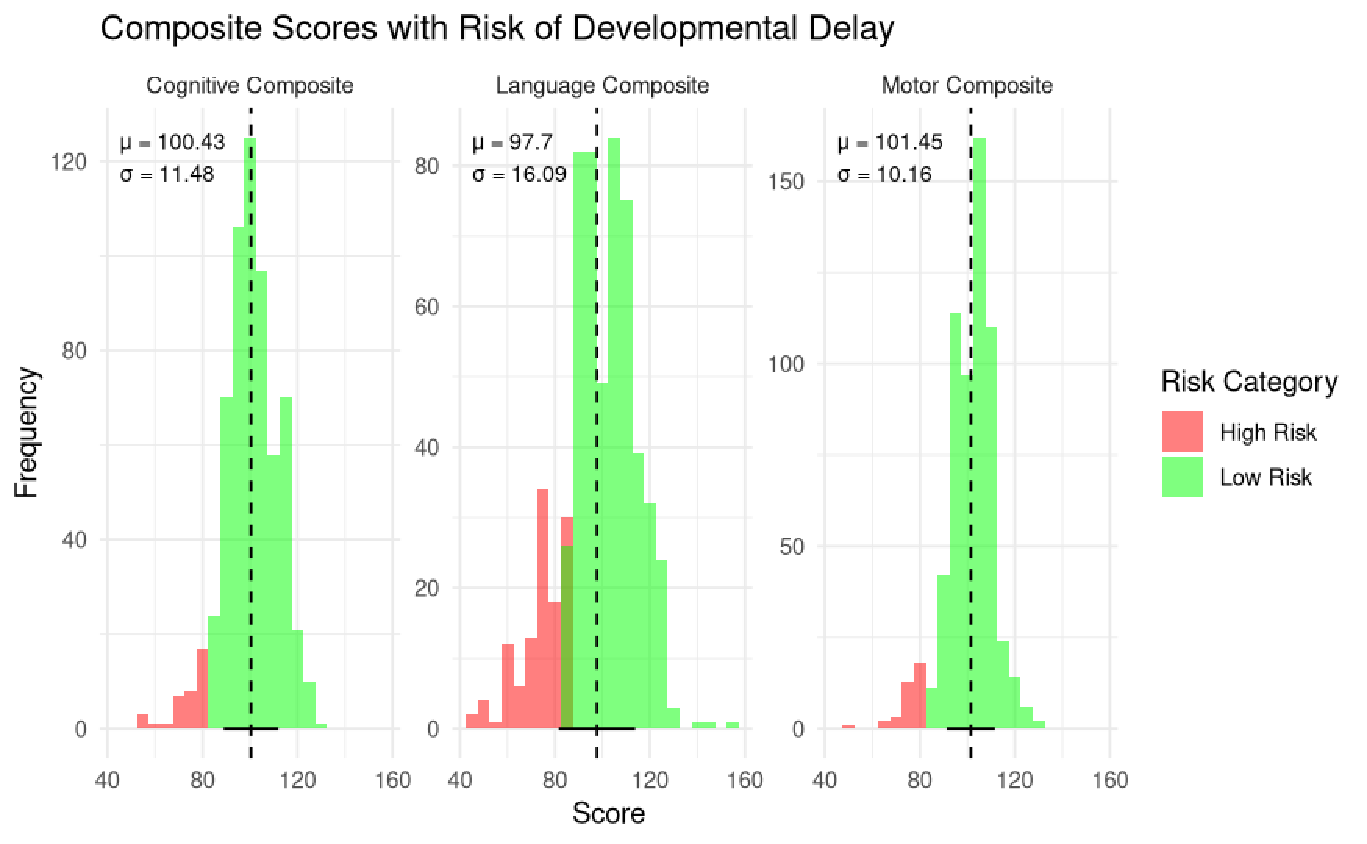
\includegraphics[width=.7\columnwidth]{img/bsid_risk.pdf}
    \caption{Distributions of composite scores based on binary classification. Assumptions made in~\cite{johnson2014using} largely hold true.}
    \label{fig:bsid-demographics}
\end{figure}

%\vspace{-0.4cm}

MRI data inside the dHCP were acquired on a 3T Philips Achieva system with a 32-channel neonatal head coil. The imaging protocol was tailored to the unique characteristics of the neonatal brain. Resting-state fMRI (rs-fMRI) was captured with a multiband-accelerated echo-planar imaging sequence (TR: 392 ms, TE: 38 ms, resolution: $2.15\text{mm}^3$) over 15 minutes (2300 volumes). The processing followed the dHCP pipeline, which is designed to address the challenges of neonatal imaging. This included motion and distortion correction, skull stripping, ICA-based denoising with FIX, and high-pass temporal filtering to remove slow drifts.
%

\subsection{Image Preprocessing}
\label{sec:preprocessing}

\subsubsection{fMRI Volumes}
To align each individual dHCP fMRI data with a neonatal-specific template space, we adopted a pipeline inspired by the automated resting-state functional framework developed for the dHCP dataset~\cite{FITZGIBBON2020117303}. Specifically, we utilized the 40-week T1-weighted template from the extended dHCP Augmented Volumetric Atlas~\cite{Schuh2018}, down-sampled from a spatial resolution of 0.5~$mm^3$ isotropic to 2.15~$mm^3$ isotropic to match the native resolution of the fMRI images. Image registration was performed using ANTs~\cite{tustison_antsx_2021} on the mean image of all time points, with the resulting transformation applied independently to each time frame in parallel. The processed outputs serve as input for the subsequent experiments.

%\subsection{Dimensionality Reduction via Group ICA}
\subsubsection{Group ICA Maps}
Additionally, we derived another input modality from processed fMRI volumes using Group Independent Component Analysis (Group ICA)~\cite{Hyvarinen1999}~\cite{Beckmann2004}. Group ICA is a widely used data-driven technique in neuroimaging that decomposes fMRI data into independent spatial and temporal components. These components represent different neural processes or functional networks. Group ICA reduces the dimensionality of the fMRI data while preserving key information and isolating biologically interpretable brain networks. These features encapsulate complex brain activity patterns in a compact representation, enhancing the expressiveness of the data and facilitating brain network-level analysis.

%\subsubsection{Preparation}
%\paragraph{Data Sampling}
%label{sec:data-sampling}

To generate the Group ICA map, we selected a subset of normally developing neonates, defined as those with cognitive, language, and motor BSID-III scores greater than 85, indicating a low risk of developmental delay, and only used these data to reduce variability and noise, ensuring a more reliable set of features.
%
Of the 739 infants with BSID scores, 431 met the criteria for normal development, with 358 having usable fMRI data. To further ensure stability, we excluded newborns with gestational ages outside 36 to 44 weeks, a range defined by the dHCP volumetric atlas~\cite{Schuh2018}, resulting in a final cohort of 348 subjects. From this group, we randomly selected 100 newborns for Group ICA analysis.

%\paragraph{Group ICA and Dimensionality Reduction}

The workflow for Group ICA and functional connectivity analysis (see Figure~\ref{fig:ica-workflow}) follows methodologies established for UKB data~\cite{ALFAROALMAGRO2018400}~\cite{Miller2016}. For the 100 selected subjects, we used MIGP (MELODIC's Incremental Group-PCA) to extract the top 1200 weighted spatial eigenvectors, approximating traditional PCA while remaining computationally efficient for large datasets~\cite{Smith2014}. Spatial Independent Component Analysis (spatial ICA) was then applied using FSL MELODIC~\cite{Hyvarinen1999}~\cite{Beckmann2004} to parcellate the data into spatially independent components (ICs). We evaluated dimensionalities of 25 and 100 ICs, consistent with previous work on the UKB dataset~\cite{ALFAROALMAGRO2018400}~\cite{Miller2016}~\cite{SMITH2013144}~\cite{doi}. Higher dimensionalities result in smaller, more numerous regions within spatial maps. Since FIX denoising was performed during preprocessing, we did not identify artifactual components.
%

Using the generated group ICA maps, we performed dual regression to obtain subject-specific spatial maps for each IC. Dual regression comprises two steps: (i) spatial regression, projecting group-level IC maps onto individual data, and (ii) temporal regression, deriving subject-specific timeseries for each IC. To further explore functional connectivity, we conducted seed-to-voxel analysis, correlating the time series of the brain regions with those of all other voxels. The resulting whole-brain functional connectivity maps served as input features for the SwiFT model to predict neurodevelopmental outcomes. We hypothesize that this approach will improve the predictive performance and the interpretability of model predictions by leveraging the reduced dimensionality and biologically relevant features.

\subsection{Evaluation Metrics}
\label{sec:evaluation_metrics}

%\paragraph{Target Developmental Outcomes}
This study focuses on predicting Bayley Scales of Infant and Toddler Development, Third Edition (Bayley-III), composite scores in cognitive, language, and motor domains from neonatal fMRI. The established thresholds for categorization of developmental delays are:

\begin{itemize}
    \item greater than or equal to 85: average development
    \item lower than 85: risk of developmental delay
    \item lower than 75: moderate to severe mental impairment~\cite{johnson2014using}
\end{itemize}

Following previous studies~\cite{he2020multi}, we simplify the classification task to a binary format, with a threshold of 85 that distinguishes low- and high-risk cases. Regression tasks are also conducted to predict continuous Bayley-III scores.

For classification tasks, we evaluate predictive performance using the area under the ROC curve (AUC), the accuracy (ACC), and the balanced accuracy (ACC$_{bal}$) to account for class imbalance. For regression tasks, we use mean absolute error (MAE) and mean squared error (MSE), along with adjusted metrics (MAE$_{adj}$ and MSE$_{adj}$) that are scaled back to the original scale of Bayley scores for better interpretability.

\subsection{Model Architecture}
\label{sec:model_architecture}
%\paragraph{Swin fMRI Transformer}  
To predict developmental outcomes using neonatal fMRI as input, we employ SwiFT, a Transformer-based model designed for high-dimensional spatiotemporal fMRI data. SwiFT processes 4D fMRI volumes by segmenting them into patches, embedding them as tokens, and passing them through layers of 4D Swin Transformer blocks. These blocks utilize a shifted window multi-head self-attention mechanism to capture both local and global spatiotemporal dependencies while minimizing computational costs through patch merging. SwiFT maintains robust performance on various tasks (e.g., predicting sex, age, intelligence, or psychiatric diagnosis), demonstrating its effectiveness in learning spatiotemporal patterns from fMRI~\cite{kim2023swiftswin4dfmri}.
%To predict developmental outcomes from neonatal fMRI, we employed SwiFT, a Transformer-based architecture designed to model high-dimensional spatiotemporal fMRI data. SwiFT processes 4D fMRI volumes, capturing local and global dependencies. The model operates by dividing 4D fMRI data into patches, embedding them as tokens, and processing these tokens through multiple layers of 4D Swin Transformer blocks. These blocks use a shifted window multi-head self-attention mechanism, enabling efficient learning of spatiotemporal patterns while reducing computational complexity through patch merging. SwiFT demonstrated robust performance on diverse tasks (e.g., predicting sex, age, intelligence, or psychiatric diagnosis), showcasing its effectiveness in learning spatiotemporal patterns from the human brains~\cite{kim2023swiftswin4dfmri}.

We train and evaluate SwiFT in an end-to-end manner from fMRI input to prediction results, with single-label and multi-label approaches: the single-label tasks involve predicting one Bayley score per input fMRI volume, while the multi-label tasks involve predicting all three Bayley scores per input fMRI volume using a shared prediction head. We hypothesize that the multi-label approach will enhance predictive performance due to the strong correlations that exist among Bayley scores (see Section~\ref{sec:dataset}), as supported by previous work~\cite{He2020}.

\subsection{Experimental Design}
\label{sec:experimental_design}

%

%(for experiemental design) Each model is fine-tuned across a predefined hyperparameter search space, including data augmentation strategies (affine-only, intensity-only, and combined transformations), learning rates, batch sizes, and patch sizes. Sequence length of the input was varied to evaluate its impact: a baseline length of 20 was used per ~\cite{kim2023swiftswin4dfmri}, with additional experiments using lengths of 50 and 100 to assess temporal dynamics, as longer sequences have shown promise in prior studies for predicting intelligence in young adults and elders~\cite{kim2023swiftswin4dfmri}.
%

%(for experimental design) To leverage publicly available fMRI datasets, we pre-trained SwiFT using contrastive self-supervised learning~\cite{dave2022TCLR} on data from the UK Biobank (UKB)~\cite{alfaro2018UKBiobank}~\cite{miller2016UKBiobank}, Human Connectome Project (HCP)~\cite{vanEssen2013HCP}, and Adolescent Brain Cognitive Development (ABCD) study~\cite{casey2018ABCD}. While this approach utilizes larger datasets, differences between neonatal and adult or adolescent brain data present potential limitations. To address size discrepancies, neonatal images were padded to 96x96x96, contrasting with experiments trained from scratch, where images were padded to 64x64x64 (see Section~\ref{sec:experimental_settings}).

%\section{Experiments}
%\label{sec:experiments}

\subsubsection{Experimental Settings}
\label{sec:experimental_settings}

All experiments were carried out on the \emph{Perlmutter} supercomputer, an HPE Cray EX system. A holdout strategy with a 70:15:15 data split was used for training, validation, and testing. To address data imbalance (see Section~\ref{sec:methods}), stratified splits were applied based on the BSID-III scores. For benchmarking, 5-fold cross-validation ensured consistent and fair splits between experiments. Hence, the metrics in this study are reported as the average over 5-fold cross-validation, with their standard deviation attached as a number with a $\pm$ sign and a smaller font.
%
For binary classification, we used weighted focal loss~\cite{lin2018focallossdenseobject} to prioritize at-risk cases that are harder to classify. This approach significantly improved performance, especially for these challenging instances.
%
Following ~\cite{kim2023swiftswin4dfmri}, we padded the input images to 64x64x64 to align with the model architecture, adapting from the 96x96x96 padding used in ~\cite{kim2023swiftswin4dfmri} due to our native image size of 45x55x45.
%
%For classification tasks, we evaluated performance using the area under the ROC curve (AUC), accuracy, and balanced accuracy (ACC$_{bal}$) to account for class imbalance. For regression tasks, mean absolute error (MAE) and mean squared error (MSE) were used, along with adjusted metrics (MAE$_{adj}$ and MSE$_{adj}$) to reflect re-scaled values for interpretability.

\subsubsection{Baselines}

We establish baseline performance using ROI-based deep learning models, including BrainNetCNN \cite{KAWAHARA20171038}, VanillaTF, and Brain Network Transformer (BNT) \cite{KAN2022}, which take functional connectivity matrices as input (computed using Pearson correlations of 87 brain regions in the neonatal brain atlas of dHCP). Hyper-parameters and implementations followed \cite{KAN2022}. Additionally, we included XGBoost \cite{CHEN2016} as a traditional machine learning baseline, using the flattened upper triangular correlation matrix as input.

\subsubsection{fMRI Volume-based Models}
\label{sec:raw_fmri}
%
SwiFT models that used fMRI volumes as inputs were fine-tuned across a predefined hyperparameter search space, including data augmentation strategies (affine-only, intensity-only, and combined transformations), learning rates, batch sizes, and patch sizes. The length of the input sequence was varied to evaluate its impact: a default length of 20 was used per ~\cite{kim2023swiftswin4dfmri}, with additional experiments using lengths of 50 and 100 to assess temporal dynamics, as longer sequences have shown promise in previous studies in predicting intelligence in young adults and elders~\cite{kim2023swiftswin4dfmri}.
%
To leverage publicly available fMRI datasets, we pre-trained SwiFT using self-supervised contrastive learning~\cite{dave2022TCLR} on data from the UK Biobank (UKB)~\cite{alfaro2018UKBiobank}~\cite{miller2016UKBiobank}, the Human Connectome Project (HCP)~\cite{vanEssen2013HCP}, and the study of Adolescent Brain Cognitive Development (ABCD)~\cite{casey2018ABCD}. Although this approach uses larger datasets, differences between newborn and adolescent/adult brain data present potential limitations. To address size discrepancies, the neonatal images were padded to 96x96x96, compared to the experiments trained from scratch, where the images were padded to 64x64x64 (see Section~\ref{sec:experimental_settings}).

%\vspace{-.7cm}

\begin{figure}[h]
    \centering
    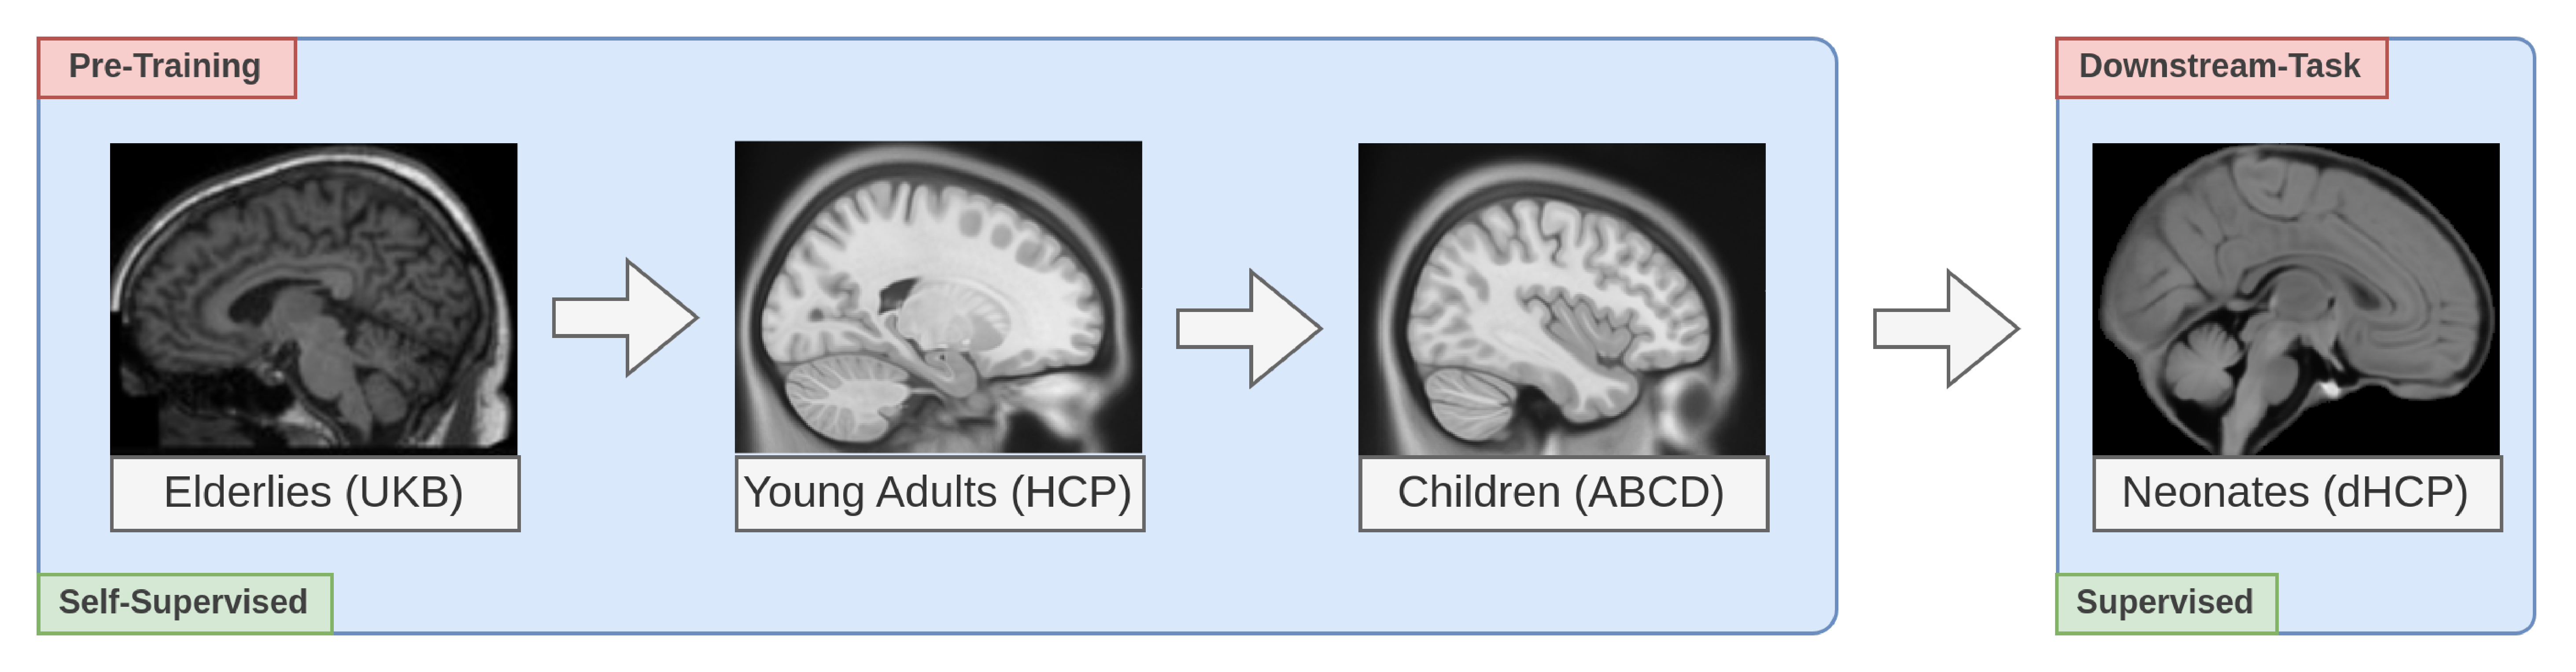
\includegraphics[width=1\columnwidth]{img/pretraining.pdf}
    \caption{Rationale of using large amounts of brain fMRI data across different datasets to make up for the little amount of data available for neonates. The expectation is that learned features from elderly, adult and child data will generalize to limited neonatal fMRI data and thus improve downstream performance for neonates.}
    \label{fig:pretraining}
\end{figure}

%\vspace{-.8cm}

\mycomment{
\subsection{Dimensionality Reduction via Group ICA}

Group Independent Component Analysis (Group ICA)~\cite{Hyvarinen1999}~\cite{Beckmann2004} is a widely used data-driven technique in neuroimaging that decomposes fMRI data into independent spatial and temporal components. These components represent distinct neural processes or functional networks. Group ICA reduces the dimensionality of high-dimensional fMRI data while preserving significant information and isolating biologically interpretable brain networks.
%
In this study, we use Group ICA features as inputs. These features encapsulate complex brain activity patterns in a compact representation, enhancing expressiveness and facilitating brain network-level analysis. We hypothesize that this approach will improve model interpretability and predictive performance by leveraging the reduced dimensionality and biologically relevant features.

\subsubsection{Preparation}
\paragraph{Data Sampling}
\label{sec:data-sampling}

To generate the Group ICA map, we selected a subset of normally developing neonates, defined as those with cognitive, language, and motor BSID-III scores above 85, indicating low risk of developmental delay. Only normally developing data were used to reduce variability and noise, ensuring a more reliable feature set.
%
Out of 725 assessed subjects, 431 met the criteria for normal development, with 358 having usable fMRI data. To further enhance stability, we excluded neonates with gestational ages outside 36 to 44 weeks, as defined by the dHCP volumetric atlas~\cite{Schuh2018}, resulting in a final cohort of 348 subjects. From this group, we randomly selected 100 neonates for Group ICA analysis.

\paragraph{Group ICA and Dimensionality Reduction}

The workflow for Group ICA and functional connectivity analysis (see Figure~\ref{fig:ica-workflow}) follows methodologies established for the UKB dataset~\cite{ALFAROALMAGRO2018400}~\cite{Miller2016}. For the selected 100 subjects, we used MIGP (MELODIC's Incremental Group-PCA) to extract the top 1200 weighted spatial eigenvectors, approximating traditional PCA while remaining computationally efficient for large datasets~\cite{Smith2014}. Spatial Independent Component Analysis (spatial-ICA) was then applied using FSL MELODIC~\cite{Hyvarinen1999}~\cite{Beckmann2004} to parcellate the data into spatially independent components (ICs). We evaluated dimensionalities of 25 and 100 ICs, consistent with prior work on the UKB dataset~\cite{ALFAROALMAGRO2018400}~\cite{Miller2016}~\cite{SMITH2013144}~\cite{doi}. Higher dimensionalities result in smaller, more numerous regions within spatial maps. Since FIX denoising was performed during preprocessing, we did not identify artifactual components.
%
Using the generated group ICA maps, we performed dual regression to obtain subject-specific spatial maps for each IC. Dual regression comprises two steps: (i) spatial regression, projecting group-level IC maps onto individual data, and (ii) temporal regression, deriving subject-specific timeseries for each IC. To further explore functional connectivity, we conducted seed-to-voxel analysis, correlating timeseries of brain regions with those of all other voxels. The resulting whole-brain functional connectivity maps served as input features for the SwiFT model to predict neurodevelopmental outcomes.
}

\begin{figure}[h]
    \centering
    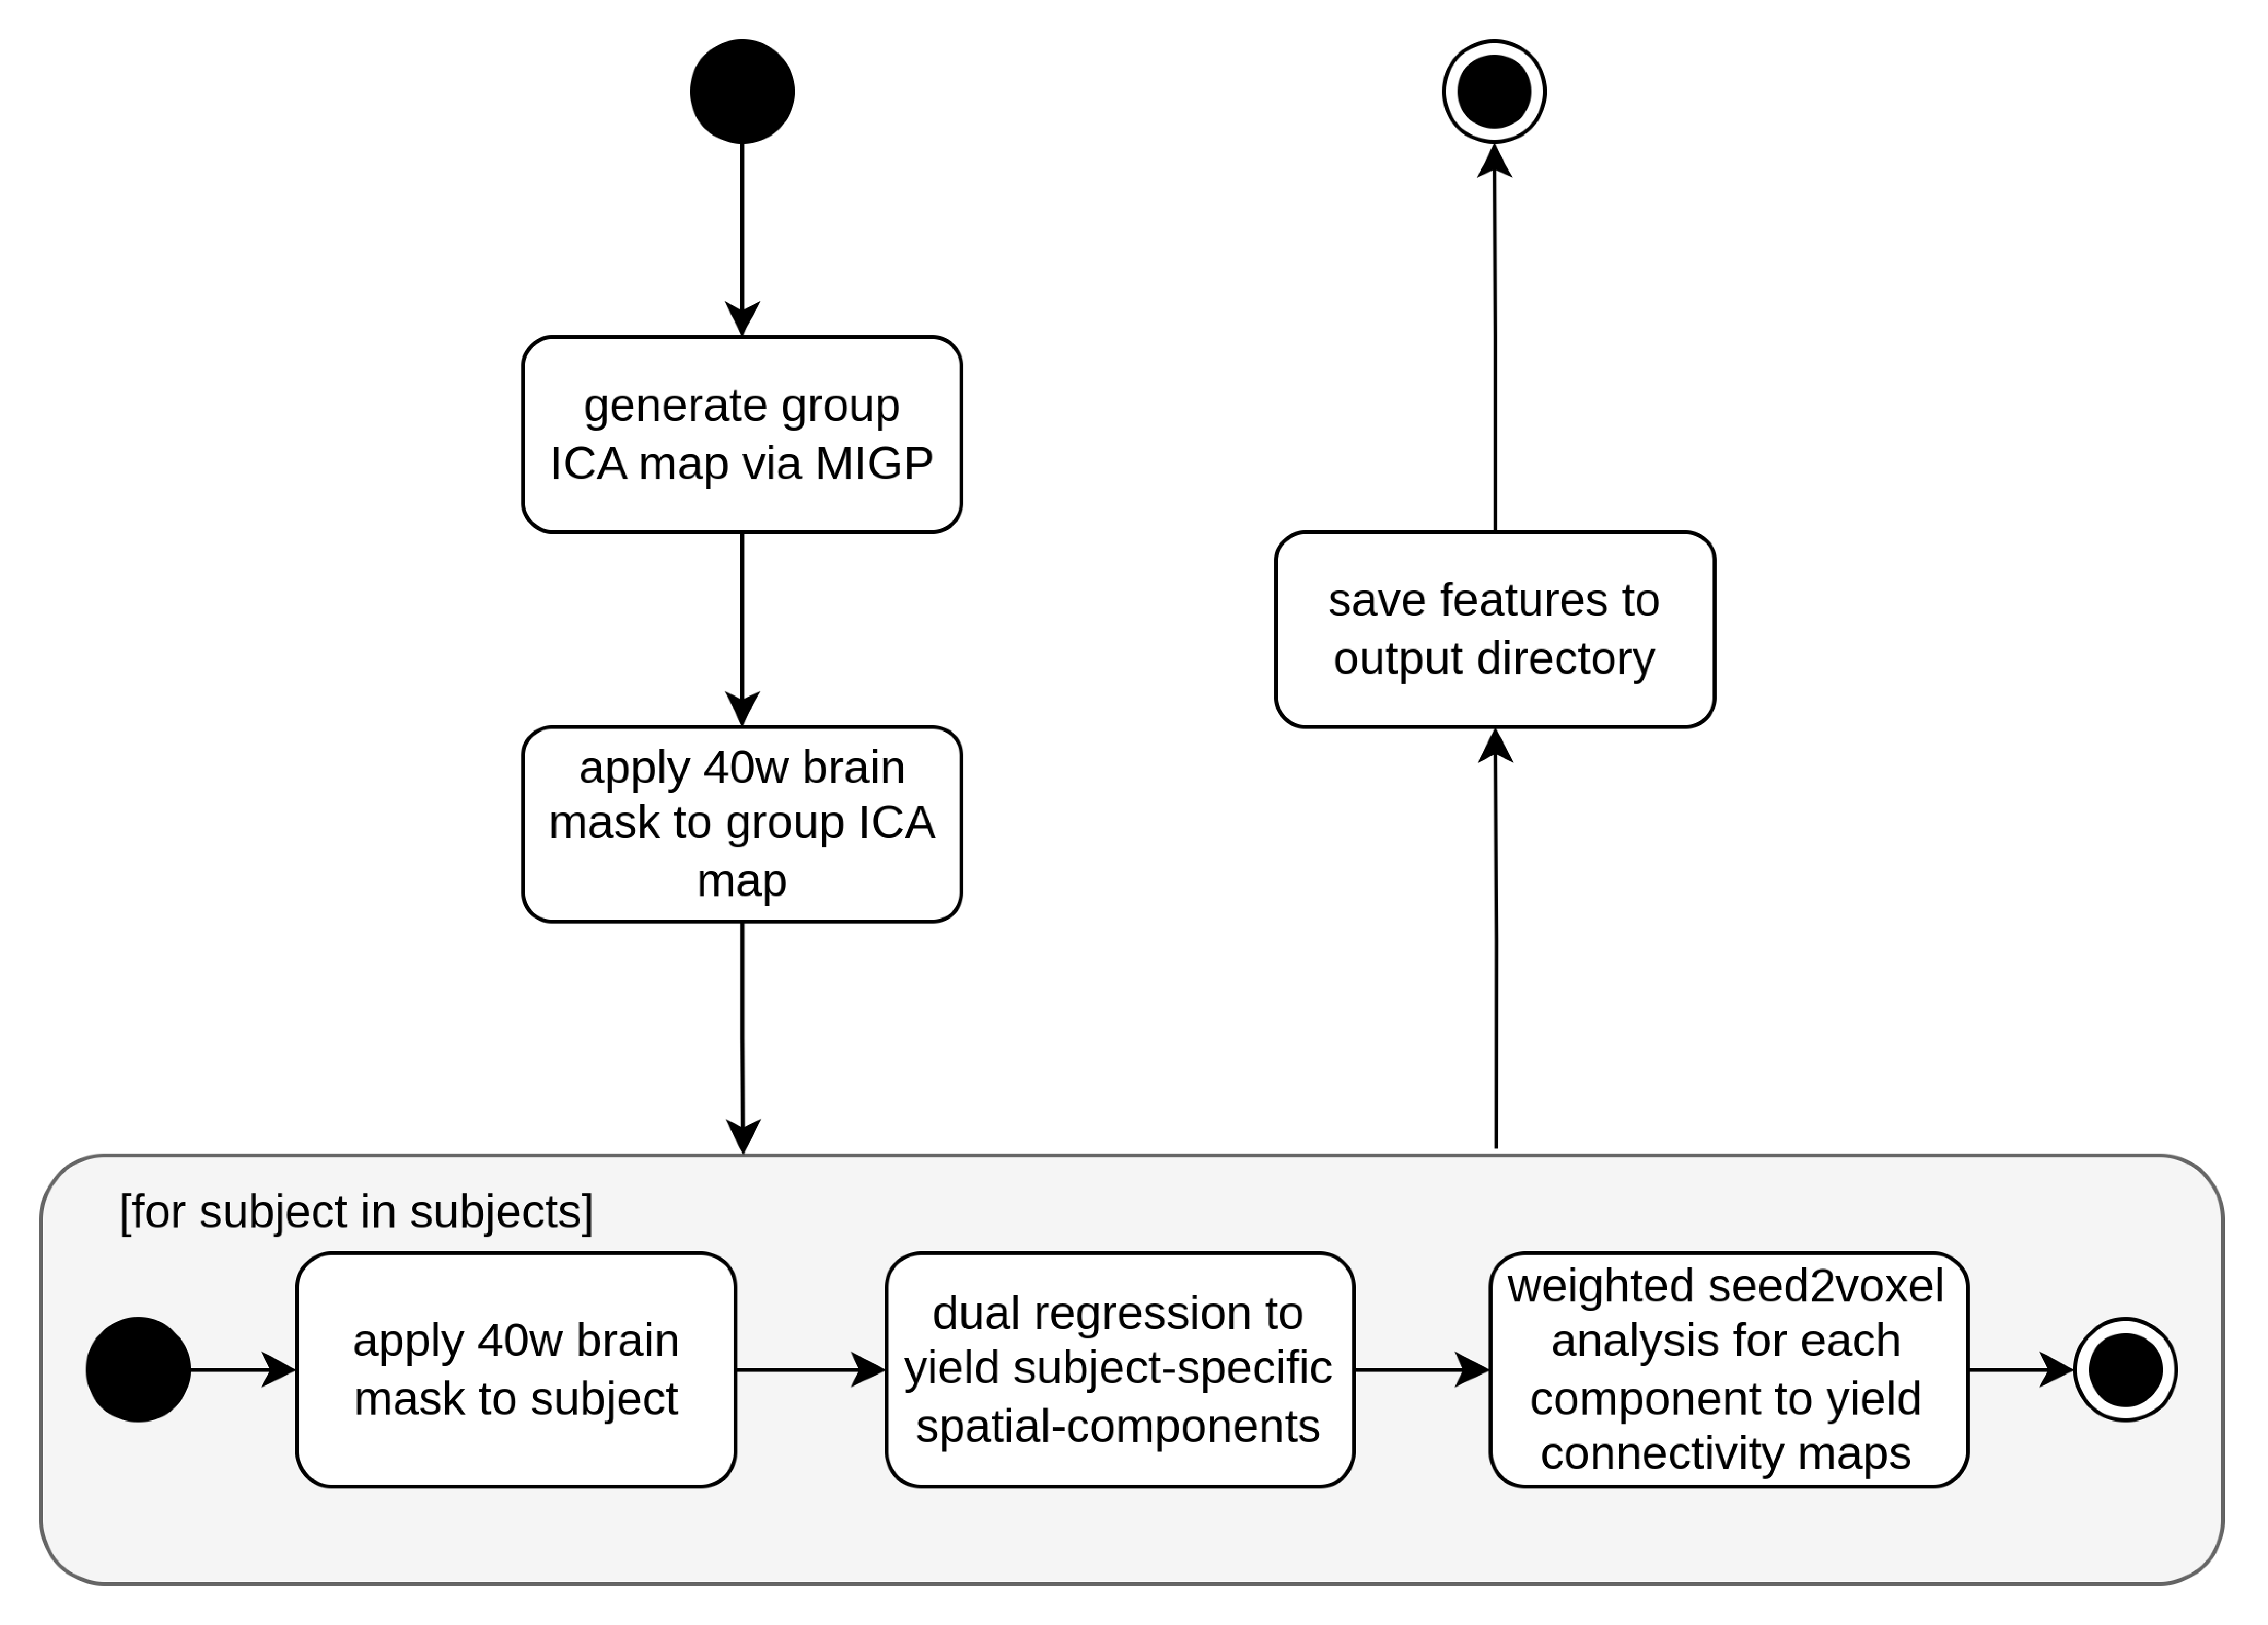
\includegraphics[width=0.5\columnwidth]{img/ica-workflow.pdf}
    \caption{UML Flowchart depicting the workflow to extract features and connectivity maps by leveraging Group Independent Component Analysis ~\cite{ALFAROALMAGRO2018400},~\cite{Miller2016} and~\cite{GAL2022118920}.}
    \label{fig:ica-workflow}
\end{figure}

%\vspace{-0.7cm}

%\subsubsection{Results}

%\paragraph{Training Process}
\subsubsection{IC-based Models}
SwiFT models that used ICA-extracted features as inputs were tuned using a predefined hyperparameter search space, including learning rate, patch size, and data augmentation strategies (see Section~\ref{sec:raw_fmri}). With ICA reducing the input data to a fraction of its original dimensionality, careful tuning was critical to ensure effective convergence. Given the data demands of transformer architectures and the reduced training data size, we increased the maximum training epochs to 100. To mitigate overfitting, we applied data augmentation techniques such as affine and intensity transformations to enhance sample diversity and improve generalizability. Due to the specific sequence lengths required for IC-based training (42 and 100), transfer learning was not utilized in these experiments.
%
To minimize bias and maintain the reliability of our experimental results, we addressed potential data leakage by ensuring that the 100 healthy subjects used for Group ICA were always included in the training set, avoiding overlap with validation or test sets.

\subsection{Attribution Analysis with Integrated Gradients}
As in ~\cite{kim2023swiftswin4dfmri}, we use Integrated Gradient with Smoothgrad sQuare (IG-SQ), implemented through the Captum framework~\cite{captum1} to identify spatial representations in brain regions that contribute to Bayley-III classification tasks.
%

For each test sample, we generated 4D IG-SQ maps and excluded misclassified instances to ensure the validity of interpretations. The resulting maps were normalized, Gaussian-smoothed, and averaged among subjects to identify spatial patterns consistently associated with cognitive, language, and motor outcomes. In addition, we aggregated these maps across ICs to derive comprehensive interpretations of brain activity relevant to each developmental domain.

\section{Results}

\subsection{Baseline Performance}
The performance of the baseline models for classification and regression can be seen in Table~\ref{tab:baseline-models}. For classification tasks, no baseline model has exceeded 52.2\% in balanced accuracy in any of the three Bayley scores, failing to significantly surpass the level of random guessing (50\%). For regression tasks, the lowest adjusted mean absolute errors reached by any baseline model for cognitive, language, and motor scores were 9.59, 13.94, and 8.55, suggesting room for improvement considering that the standard deviation of these scores were 11.48, 16.09, and 10.16, as seen in Figure~\ref{fig:bsid-demographics}.

%\vspace{-.6cm}

\begin{table}[h]
\centering
\caption{Baseline performances on regression (left) and classification (right).}
\label{tab:baseline-models}

\begin{minipage}{0.45\textwidth}
%\scriptsize % Reduce font size
\resizebox{\textwidth}{!}{%
\begin{tabular}{|l|c|c|c|}
\hline
\multirow{2}{*}{Model} & \multicolumn{3}{c|}{Cog} \\ \cline{2-4} 
 & $\text{MSE}_{\text{adj}}$ & MAE & $\text{MAE}_{\text{adj}}$ \\ \hline
XGBoost & $155.6_{\pm15.0}$ & $\mathbf{0.84_{\pm0.03}}$ & $\mathbf{9.59_{\pm0.48}}$ \\ \hline
BrainNetCNN & $\mathbf{113.6_{\pm54.2}}$ & $0.84_{\pm0.09}$ & $9.66_{\pm1.55}$ \\ \hline
VanillaTF & $210.1_{\pm91.4}$ & $0.91_{\pm0.04}$ & $10.43_{\pm1.13}$ \\ \hline
BNT & $147.1_{\pm86.7}$ & $0.87_{\pm0.07}$ & $10.01_{\pm1.33}$ \\ \hline
\end{tabular}
}

\vspace{.3em}

\resizebox{\textwidth}{!}{%
\begin{tabular}{|l|c|c|c|}
\hline
\multirow{2}{*}{Model} & \multicolumn{3}{c|}{Lang} \\ \cline{2-4} 
 & $\text{MSE}_{\text{adj}}$ & MAE & $\text{MAE}_{\text{adj}}$ \\ \hline
XGBoost & $304.7_{\pm33.9}$ & $\mathbf{0.86_{\pm0.07}}$ & $\mathbf{13.94_{\pm0.75}}$ \\ \hline
BrainNetCNN & $317.6_{\pm109.6}$ & $0.88_{\pm0.04}$ & $14.28_{\pm1.31}$ \\ \hline
VanillaTF & $\mathbf{279.7_{\pm96.3}}$ & $0.91_{\pm0.03}$ & $14.77_{\pm1.21}$ \\ \hline
BNT & $355.1_{\pm49.6}$ & $0.90_{\pm0.03}$ & $14.68_{\pm1.20}$ \\ \hline
\end{tabular}
}

\vspace{.3em}

\resizebox{\textwidth}{!}{%
\begin{tabular}{|l|c|c|c|}
\hline
\multirow{2}{*}{Model} & \multicolumn{3}{c|}{Mot} \\ \cline{2-4} 
 & $\text{MSE}_{\text{adj}}$ & MAE & $\text{MAE}_{\text{adj}}$ \\ \hline
XGBoost & $124.9_{\pm18.0}$ & $\mathbf{0.81_{\pm0.05}}$ & $\mathbf{8.55_{\pm0.59}}$ \\ \hline
BrainNetCNN & $\mathbf{115.74_{\pm28.5}}$ & $0.84_{\pm0.04}$ & $8.93_{\pm0.75}$ \\ \hline
VanillaTF & $173.0_{\pm108.2}$ & $0.86_{\pm0.03}$ & $9.11_{\pm0.84}$ \\ \hline
BNT & $153.7_{\pm100.4}$ & $0.81_{\pm0.04}$ & $8.58_{\pm0.90}$ \\ \hline
\end{tabular}
}
\end{minipage}
%hfill
\hspace{3em}
\begin{minipage}{0.4\textwidth}

\resizebox{\textwidth}{!}{%
\begin{tabular}{|l|c|c|c|}
\hline
\multirow{2}{*}{Model} & \multicolumn{3}{c|}{Cog} \\ \cline{2-4} 
 & $\text{ACC}_{\text{bal}}$ & ACC & AUC \\ \hline
XGBoost & $50.0_{\pm0.0}$ & $\mathbf{93.8_{\pm0.4}}$ & $51.5_{\pm10.4}$ \\ \hline
BrainNetCNN & $49.6_{\pm0.4}$ & $93.0_{\pm1.0}$ & $47.5_{\pm4.8}$ \\ \hline
VanillaTF & $\mathbf{52.2_{\pm4.2}}$ & $92.5_{\pm1.0}$ & $55.5_{\pm9.5}$ \\ \hline
BNT & $51.2_{\pm3.7}$ & $93.1_{\pm1.0}$ & $\mathbf{59.8_{\pm4.2}}$ \\ \hline
\end{tabular}
}

\vspace{.3em}

\resizebox{\textwidth}{!}{%
\begin{tabular}{|l|c|c|c|}
\hline
\multirow{2}{*}{Model} & \multicolumn{3}{c|}{Lang} \\ \cline{2-4} 
 & $\text{ACC}_{\text{bal}}$ & ACC & AUC \\ \hline
XGBoost & $50.0_{\pm0.9}$ & $\mathbf{79.5_{\pm0.8}}$ & $50.4_{\pm7.5}$ \\ \hline
BrainNetCNN & $50.3_{\pm3.0}$ & $77.5_{\pm3.1}$ & $\mathbf{56.1_{\pm4.9}}$ \\ \hline
VanillaTF & $49.9_{\pm2.4}$ & $74.0_{\pm2.4}$ & $54.1_{\pm6.8}$ \\ \hline
BNT & $\mathbf{51.1_{\pm3.9}}$ & $74.8_{\pm3.1}$ & $\mathbf{57.1_{\pm5.6}}$ \\ \hline
\end{tabular}
}

\vspace{.3em}

\resizebox{\textwidth}{!}{%
\begin{tabular}{|l|c|c|c|}
\hline
\multirow{2}{*}{Model} & \multicolumn{3}{c|}{Mot} \\ \cline{2-4} 
 & $\text{ACC}_{\text{bal}}$ & ACC & AUC \\ \hline
XGBoost & $\mathbf{49.7_{\pm0.3}}$ & $\mathbf{93.1_{\pm0.5}}$ & $51.2_{\pm6.2}$ \\ \hline
BrainNetCNN & $49.5_{\pm0.7}$ & $92.7_{\pm1.3}$ & $\mathbf{57.1_{\pm5.6}}$ \\ \hline
VanillaTF & $49.2_{\pm0.4}$ & $92.1_{\pm0.8}$ & $47.4_{\pm7.9}$ \\ \hline
BNT & $49.5_{\pm0.3}$ & $92.7_{\pm0.7}$ & $44.7_{\pm6.8}$ \\ \hline
\end{tabular}
}
\end{minipage}

\end{table}

%\vspace{-1cm}

\subsection{fMRI Volume-based Model Performance}

\subsubsection{Single-label Prediction}

The choice of sequence length had a notable impact on the model's performance. A length of 50 yielded the best results, while shorter (20) or longer (100) sequences performed slightly worse, suggesting that an optimal balance is necessary. The displayed results are from models with the best performing set of hyperparameters.
%
As shown in Table~\ref{tab:bsid-raw}, pre-training resulted in marginal improvements in predictive power for BSID-III scores. However, increased padding to fit the pre-trained network architecture might have negatively influenced the performance. Compared to baseline models, SwiFT yielded significant performance gains for both regression and classification tasks. For cognitive and language predictions, adjusted MAE improved by approximately 11\%, while gains for motor regression were minimal. In classification, the balanced accuracy ($\text{ACC}_{bal}$) improved by around 5\%p, significantly exceeding the random guess range.

\begin{table}[h]
\centering
\caption{SwiFT’s performance with raw fMRI as input on single-label (left) and multi-label (right) predictions.}
\label{tab:bsid-raw}

\begin{minipage}{0.4\textwidth}
\resizebox{\textwidth}{!}{%
\begin{tabular}{|l|c|c|c|}
\hline
\multirow{2}{*}{Method} & \multicolumn{3}{c|}{Cog} \\ \cline{2-4} 
 & $\text{MSE}_{adj}$ & MAE & $\text{MAE}_{adj}$ \\ \hline
Scratch & $127.8_{\pm11.8}$ & $0.77_{\pm0.03}$ & $8.8_{\pm0.7}$ \\\hline
Pre-Tr. & $\mathbf{123.5_{\pm12.6}}$ & $\mathbf{0.76_{\pm0.02}}$ & $\mathbf{8.6_{\pm0.5}}$ \\ \hline
%\multicolumn{7}{c}{\mbox{ }} \\ 
\hline
 & ACC & $\text{ACC}_{bal}$ & AUC \\ \hline
Scratch & $94.4_{\pm0.7}$ & $\mathbf{54.9_{\pm3.8}}$ & $\mathbf{56.9_{\pm5.2}}$ \\ \hline
Pre-Tr. & $\mathbf{94.9_{\pm1.2}}$ & $54.1_{\pm3.6}$ & $54.6_{\pm3.2}$ \\
\hline
\end{tabular}
}

\vspace{.3em}

\resizebox{\textwidth}{!}{%
\begin{tabular}{|l|c|c|c|}
\hline
\multirow{2}{*}{Method} & \multicolumn{3}{c|}{Lang} \\ \cline{2-4} 
 & $\text{MSE}_{adj}$ & MAE & $\text{MAE}_{adj}$ \\ \hline
Scratch & $293.4_{\pm20.1}$ & $0.79_{\pm0.04}$ & $12.9_{\pm0.5}$ \\ \hline
Pre-Tr. & $\mathbf{287.4_{\pm15.4}}$ & $\mathbf{0.78_{\pm0.02}}$ & $\mathbf{12.6_{\pm0.3}}$ \\ \hline
%\multicolumn{4}{c}{\mbox{ }} \\ 
\hline
 & ACC & $\text{ACC}_{bal}$ & AUC \\ \hline
Scratch & $82.7_{\pm2.8}$ & $56.2_{\pm2.1}$ & $\mathbf{56.6_{\pm3.2}}$ \\ \hline
Pre-Tr. & $\mathbf{83.9_{\pm1.4}}$ & $\mathbf{57.6_{\pm3.1}}$ & $56.3_{\pm3.1}$ \\ \hline
\end{tabular}
}

\vspace{.3em}

\resizebox{\textwidth}{!}{%
\begin{tabular}{|l|c|c|c|}
\hline
\multirow{2}{*}{Method} & \multicolumn{3}{c|}{Mot} \\ \cline{2-4} 
 & $\text{MSE}_{adj}$ & MAE & $\text{MAE}_{adj}$ \\ \hline
Scratch & $\mathbf{103.1_{\pm9.2}}$  & $\mathbf{0.81_{\pm0.08}}$  & $\mathbf{8.4_{\pm0.9}}$ \\ \hline
Pre-Tr. & $105.7_{\pm9.8}$  & $0.82_{\pm0.09}$  & $8.6_{\pm1.1}$ \\ \hline
%\multicolumn{4}{c}{\mbox{ }} \\ 
\hline
 & ACC & $\text{ACC}_{bal}$ & AUC \\ \hline
Scratch & $\mathbf{93.6_{\pm0.6}}$  & $54.2_{\pm3.2}$  & $55.5_{\pm3.7}$ \\ \hline
Pre-Tr. & $92.8_{\pm1.2}$  & $\mathbf{55.1_{\pm3.3}}$  & $\mathbf{55.7_{\pm3.9}}$ \\ \hline
\end{tabular}
}
\end{minipage}
\hspace{3em}
\begin{minipage}{0.4\textwidth}
\resizebox{\textwidth}{!}{%
\begin{tabular}{|l|c|c|c|}
\hline
\multirow{2}{*}{Method} & \multicolumn{3}{c|}{Cog} \\ \cline{2-4} 
 & $\text{MSE}_{adj}$ & MAE & $\text{MAE}_{adj}$ \\ \hline
Scratch & $125.7_{\pm16.6}$ & $\mathbf{0.64_{\pm0.07}}$ & $\mathbf{8.5_{\pm0.6}}$ \\\hline
Pre-Tr. & $\mathbf{119.2_{\pm12.6}}$ & $0.64_{\pm0.12}$ & $8.6_{\pm1.2}$ \\ \hline
%\multicolumn{7}{c}{\mbox{ }} \\ 
\hline
 & ACC & $\text{ACC}_{bal}$ & AUC\\ \hline
Scratch & $\mathbf{96.4_{\pm1.0}}$ & $59.7_{\pm2.1}$ & $62.6_{\pm4.0}$ \\ \hline
Pre-Tr. & $95.6_{\pm2.4}$ & $\mathbf{66.0_{\pm2.9}}$ & $\mathbf{62.7_{\pm4.7}}$ \\
\hline
\end{tabular}
}

\vspace{.3em}

\resizebox{\textwidth}{!}{%
\begin{tabular}{|l|c|c|c|}
\hline
\multirow{2}{*}{Method} & \multicolumn{3}{c|}{Lang} \\ \cline{2-4} 
 & $\text{MSE}_{adj}$ & MAE & $\text{MAE}_{adj}$ \\ \hline
Scratch & $212.4_{\pm17.7}$ & $0.87_{\pm0.05}$ & $11.6_{\pm0.7}$ \\ \hline
Pre-Tr. & $\mathbf{205.3_{\pm15.3}}$ & $\mathbf{0.86_{\pm0.07}}$ & $\mathbf{11.5_{\pm0.9}}$ \\ \hline
%\multicolumn{4}{c}{\mbox{ }} \\ 
\hline
 & ACC & $\text{ACC}_{bal}$ & AUC \\ \hline
Scratch & $83.3_{\pm1.5}$ & $61.7_{\pm1.7}$ & $62.0_{\pm1.9}$ \\ \hline
Pre-Tr. & $\mathbf{83.7_{\pm1.3}}$ & $\mathbf{62.3_{\pm1.9}}$ & $\mathbf{63.2_{\pm2.2}}$ \\ \hline
\end{tabular}
}

\vspace{.3em}

\resizebox{\textwidth}{!}{%
\begin{tabular}{|l|c|c|c|}
\hline
\multirow{2}{*}{Method} & \multicolumn{3}{c|}{Mot} \\ \cline{2-4} 
 & $\text{MSE}_{adj}$ & MAE & $\text{MAE}_{adj}$ \\ \hline
Scratch & $\mathbf{99.8_{\pm15.3}}$  & $\mathbf{0.56_{\pm0.03}}$  & $\mathbf{7.4_{\pm0.5}}$ \\ \hline
Pre-Tr. & $103.0_{\pm13.2}$  & $0.57_{\pm0.04}$  & $7.6_{\pm0.6}$ \\ \hline
%\multicolumn{4}{c}{\mbox{ }} \\ 
\hline
 & ACC & $\text{ACC}_{bal}$ & AUC \\ \hline
Scratch & $95.2_{\pm0.7}$  & $\mathbf{57.8_{\pm2.1}}$  & $\mathbf{59.7_{\pm1.7}}$ \\ \hline
Pre-Tr. & $\mathbf{95.2_{\pm0.5}}$ & $56.3_{\pm1.9}$  & $58.9_{\pm1.9}$ \\ \hline
\end{tabular}
}
\end{minipage}

\end{table}

\subsubsection{Multi-label Prediction}

Changing sequence length showed similar effects to single-label predictions. As shown in Table~\ref{tab:bsid-raw}, pre-training provided marginal improvements, suggesting limited transferability of adult data to neonatal predictions. However, multi-label prediction results show performance gains across all classes for both regression and classification, aligning with previous studies~\cite{He2020}.

\subsection{IC-based Model Performance}
\subsubsection{Single-label Prediction}
The results shown in Table \ref{tab:bsid-ica} indicate that the ICA dimensionality (25 vs. 100 ICs) does not significantly impact performance, suggesting that ICA robustly captures essential neural features regardless of the number of components. Furthermore, single-label learning with ICA-extracted features outperformed raw fMRI predictions, particularly for language classification and motor regression tasks.
%
\subsubsection{Multi-label Prediction}
The combination of ICA and multi-label learning further enhanced predictive power, aligning with previous findings on the interrelated nature of developmental outcomes.


\begin{table}[h]
\centering
\caption{SwiFT’s performance with IC-extracted features as input on single-label (left) and multi-label (right) predictions.}
\label{tab:bsid-ica}

\begin{minipage}{0.4\textwidth}
\resizebox{\textwidth}{!}{%
\begin{tabular}{|l|c|c|c|}
\hline
\multirow{2}{*}{ICs} & \multicolumn{3}{c|}{Cog} \\ \cline{2-4} 
 & $\text{MSE}_{adj}$ & MAE & $\text{MAE}_{adj}$ \\ \hline
25 & $127.2_{\pm6.9}$  & $\mathbf{0.74_{\pm0.03}}$  & $\mathbf{8.7_{\pm0.4}}$ \\ \hline
100 & $\mathbf{126.8_{\pm8.2}}$  & $0.74_{\pm0.07}$ & $8.7_{\pm0.9}$ \\ \hline
%\multicolumn{7}{c}{\mbox{ }} \\ 
\hline
 & ACC & $\text{ACC}_{bal}$ & AUC \\ \hline
25 & $93.7_{\pm1.5}$ & $\mathbf{55.7_{\pm4.0}}$ & $\mathbf{56.6_{\pm4.7}}$ \\ \hline
100 & $\mathbf{93.8_{\pm1.3}}$ & $52.4_{\pm1.2}$  & $53.1_{\pm2.4}$ \\ \hline
\end{tabular}
}

\vspace{.3em}

\resizebox{\textwidth}{!}{%
\begin{tabular}{|l|c|c|c|}
\hline
\multirow{2}{*}{ICs} & \multicolumn{3}{c|}{Lang} \\ \cline{2-4} 
 & $\text{MSE}_{adj}$ & MAE & $\text{MAE}_{adj}$ \\ \hline
25 & $\mathbf{293.4_{\pm11.4}}$ & $0.82_{\pm0.02}$  & $12.6_{\pm0.3}$ \\ \hline
100 & $299.5_{\pm13.3}$ & $\mathbf{0.8_{\pm0.02}}$ & $\mathbf{12.4_{\pm0.3}}$ \\ \hline
%\multicolumn{4}{c}{\mbox{ }} \\ 
\hline
 & ACC & $\text{ACC}_{bal}$ & AUC \\ \hline
25 & $\mathbf{84.0_{\pm2.9}}$ & $\mathbf{57.8_{\pm2.3}}$ & $\mathbf{58.3_{\pm2.8}}$ \\ \hline
100 & $82.5_{\pm3.5}$ & $56.3_{\pm1.8}$ & $57.2_{\pm2.4}$ \\ \hline
\end{tabular}
}

\vspace{.3em}

\resizebox{\textwidth}{!}{%
\begin{tabular}{|l|c|c|c|}
\hline
\multirow{2}{*}{ICs} & \multicolumn{3}{c|}{Mot} \\ \cline{2-4} 
 & $\text{MSE}_{adj}$ & MAE & $\text{MAE}_{adj}$ \\ \hline
25 & $95.7_{\pm9.2}$  & $0.76_{\pm0.04}$  & $7.7_{\pm0.3}$ \\ \hline
100 & $\mathbf{94.0_{\pm10.3}}$  & $\mathbf{0.75_{\pm0.03}}$ & $\mathbf{7.5_{\pm0.2}}$ \\ \hline
%\multicolumn{4}{c}{\mbox{ }} \\ 
\hline
 & ACC & $\text{ACC}_{bal}$ & AUC \\ \hline
25 & $\mathbf{95.2_{\pm0.7}}$ & $55.3_{\pm3.6}$ & $56.1_{\pm3.8}$ \\ \hline
100 & $92.8_{\pm0.9}$ & $\mathbf{55.6_{\pm3.1}}$ & $\mathbf{56.7_{\pm3.4}}$ \\ \hline
\end{tabular}
}
\end{minipage}
\hspace{3em}
\begin{minipage}{0.4\textwidth}
\resizebox{\textwidth}{!}{%
\begin{tabular}{|l|c|c|c|}
\hline
\multirow{2}{*}{ICs} & \multicolumn{3}{c|}{Cog} \\ \cline{2-4} 
 & $\text{MSE}_{adj}$ & MAE & $\text{MAE}_{adj}$ \\ \hline
25 & $\mathbf{119.8_{\pm10.9}}$ & $\mathbf{0.61_{\pm0.06}}$ & $\mathbf{8.1_{\pm0.55}}$ \\\hline
100 & $121.1_{\pm7.0}$ & $0.65_{\pm0.07}$ & $8.6_{\pm0.8}$ \\ \hline
%\multicolumn{7}{c}{\mbox{ }} \\ 
\hline
 & ACC & $\text{ACC}_{bal}$ & AUC \\ \hline
25 & $95.0_{\pm1.4}$ & $\mathbf{60.6_{\pm1.6}}$  & $\mathbf{62.2_{\pm1.6}}$ \\ \hline
100 & $\mathbf{95.8_{\pm1.3}}$ & $59.4_{\pm1.8}$ & $61.6_{\pm1.4}$ \\
\hline
\end{tabular}
}

\vspace{.3em}

\resizebox{\textwidth}{!}{%
\begin{tabular}{|l|c|c|c|}
\hline
\multirow{2}{*}{ICs} & \multicolumn{3}{c|}{Lang} \\ \cline{2-4} 
 & $\text{MSE}_{adj}$ & MAE & $\text{MAE}_{adj}$ \\ \hline
25 & $\mathbf{212.1_{\pm17.2}}$ & $\mathbf{0.85_{\pm0.02}}$ & $\mathbf{11.4_{\pm0.4}}$ \\ \hline
100 & $221.1_{\pm20.4}$ & $0.86_{\pm0.03}$  & $11.5_{\pm0.5}$ \\ \hline
%\multicolumn{4}{c}{\mbox{ }} \\ 
\hline
 & ACC & $\text{ACC}_{bal}$ & AUC \\ \hline
25 & $\mathbf{83.9_{\pm2.6}}$  & $62.2_{\pm0.9}$  & $62.9_{\pm1.2}$ \\ \hline
100 & $81.3_{\pm3.3}$ & $\mathbf{62.7_{\pm1.3}}$  & $\mathbf{63.8_{\pm1.7}}$ \\ \hline
\end{tabular}
}

\vspace{.3em}

\resizebox{\textwidth}{!}{%
\begin{tabular}{|l|c|c|c|}
\hline
\multirow{2}{*}{ICs} & \multicolumn{3}{c|}{Mot} \\ \cline{2-4} 
 & $\text{MSE}_{adj}$ & MAE & $\text{MAE}_{adj}$ \\ \hline
25 & $\mathbf{90.1_{\pm9.6}}$ & $\mathbf{0.53_{\pm0.04}}$ & $\mathbf{7.0_{\pm0.5}}$ \\ \hline
100 & $90.3_{\pm10.5}$ & $0.55_{\pm0.04}$  & $7.1_{\pm0.6}$ \\ \hline
%\multicolumn{4}{c}{\mbox{ }} \\ 
\hline
 & ACC & $\text{ACC}_{bal}$ & AUC \\ \hline
25 & $94.5_{\pm1.3}$  & $\mathbf{58.4_{\pm1.5}}$ & $\mathbf{60.1_{\pm1.7}}$ \\ \hline
100 & $\mathbf{95.0_{\pm1.5}}$ & $57.2_{\pm2.1}$ & $59.7_{\pm1.5}$ \\ \hline
\end{tabular}
}
\end{minipage}
\end{table}



%This study demonstrates that integrating Group ICA-based dimensionality reduction with the SwiFT Transformer architecture significantly enhances the prediction of neurodevelopmental outcomes from neonatal fMRI data. By extracting biologically meaningful features through ICA and employing multi-label learning, our approach balances dimensionality reduction with the preservation of critical neural information. The SwiFT Transformer uniquely learns complex spatiotemporal patterns in early brain development directly from 4D fMRI data, leveraging its attention-based architecture to model both local and global dependencies. These findings highlight the potential of combining neuroscience-driven feature engineering with advanced machine learning to improve both interpretability and predictive accuracy, providing a robust framework for neurodevelopmental research and clinical applications.
%
%Our results indicate that the choice of ICA dimensionality (25 vs. 100 ICs) does not significantly affect the model's predictive performance in regression or classification tasks. This invariance suggests that ICA robustly captures the essential features of neural activity, regardless of the specific number of components used. Both configurations effectively isolate key brain networks while filtering out noise, ensuring that critical information relevant to neurodevelopmental outcomes is retained. This finding reinforces the adaptability of ICA-based dimensionality reduction as a reliable preprocessing step for fMRI analysis.
%
%As shown in Table~\ref{tab:bsid-ica}, single-label learning with ICA-extracted features slightly outperforms predictions using raw fMRI data, particularly for language skill classification and motor skill regression. These results demonstrate that dimensionality reduction through ICA retains critical neural information while effectively filtering out noise. By isolating independent components that likely represent functional networks related to cognitive, language, and motor development, ICA enables the model to better capture the neural patterns underlying developmental outcomes. This process not only preserves essential details but also reduces the computational complexity associated with high-dimensional raw data.
%
%Furthermore, ICA’s ability to extract biologically meaningful components allows the model to focus on critical brain networks, improving accuracy and robustness over using the more variable and noisy raw data. This targeted approach highlights the value of combining neuroscience-driven feature engineering with advanced machine learning methods. When paired with multi-label learning, as shown in Table~\ref{tab:bsid-ica}, ICA-extracted features yield the best results, demonstrating similar performance boosts to those observed with raw fMRI volumes. This underscores the effectiveness of integrating ICA into our pipeline to enhance predictive power and model efficiency.

\subsection{Comparative Analysis}

%We have summarized our experimental results via boxplots in Figure~\ref{fig:overview}, while omitting results obtained via transfer-learning and higher-dimensional ICs due to no statistically significant performance changes. Across all metrics, Multi-ICA demonstrates significant and consistent improvements over the best-performing baseline model for most tasks, particularly in Cognitive MAE (\textit{p} = 0.004) and Motor MAE (\textit{p} = 0.002). These results underscore the advantage of incorporating ICA-extracted features in the regression of cognitive and motor delays.

We summarize our experimental results using boxplots in Figure~\ref{fig:overview}, while omitting results obtained through transfer learning and higher dimensional ICs due to the absence of statistically significant performance changes. After statistical significance analysis between the best performing baseline model and SwiFT variation for each task on all metrics, Multi-ICA demonstrates significant and consistent improvements over the baseline model for most tasks, and these improvements are especially pronounced in cognitive MAE ($p = 0.004$) and motor MAE ($p = 0.002$). 
%
Similarly, for regression tasks, Multi-ICA achieved significant reductions in cognitive regression $\text{MSE}_{adj}$ (\textit{p} = 0.036) and language regression $\text{MSE}_{adj}$ (\textit{p} = 0.008) compared to baselines.
%
In classification, Multi-ICA also achieves significant improvements in language classification accuracy (\textit{p} = 0.004) and motor classification AUC (\textit{p} = 0.044), while maintaining competitive performance in most other metrics. However, some metrics such as AUC in
the classification of cognitive scores (\textit{p} = 0.413) did not show statistically significant differences compared to the baseline.
%


\begin{figure}[h]
    \centering
    \begin{minipage}{0.45\textwidth}
        \centering
        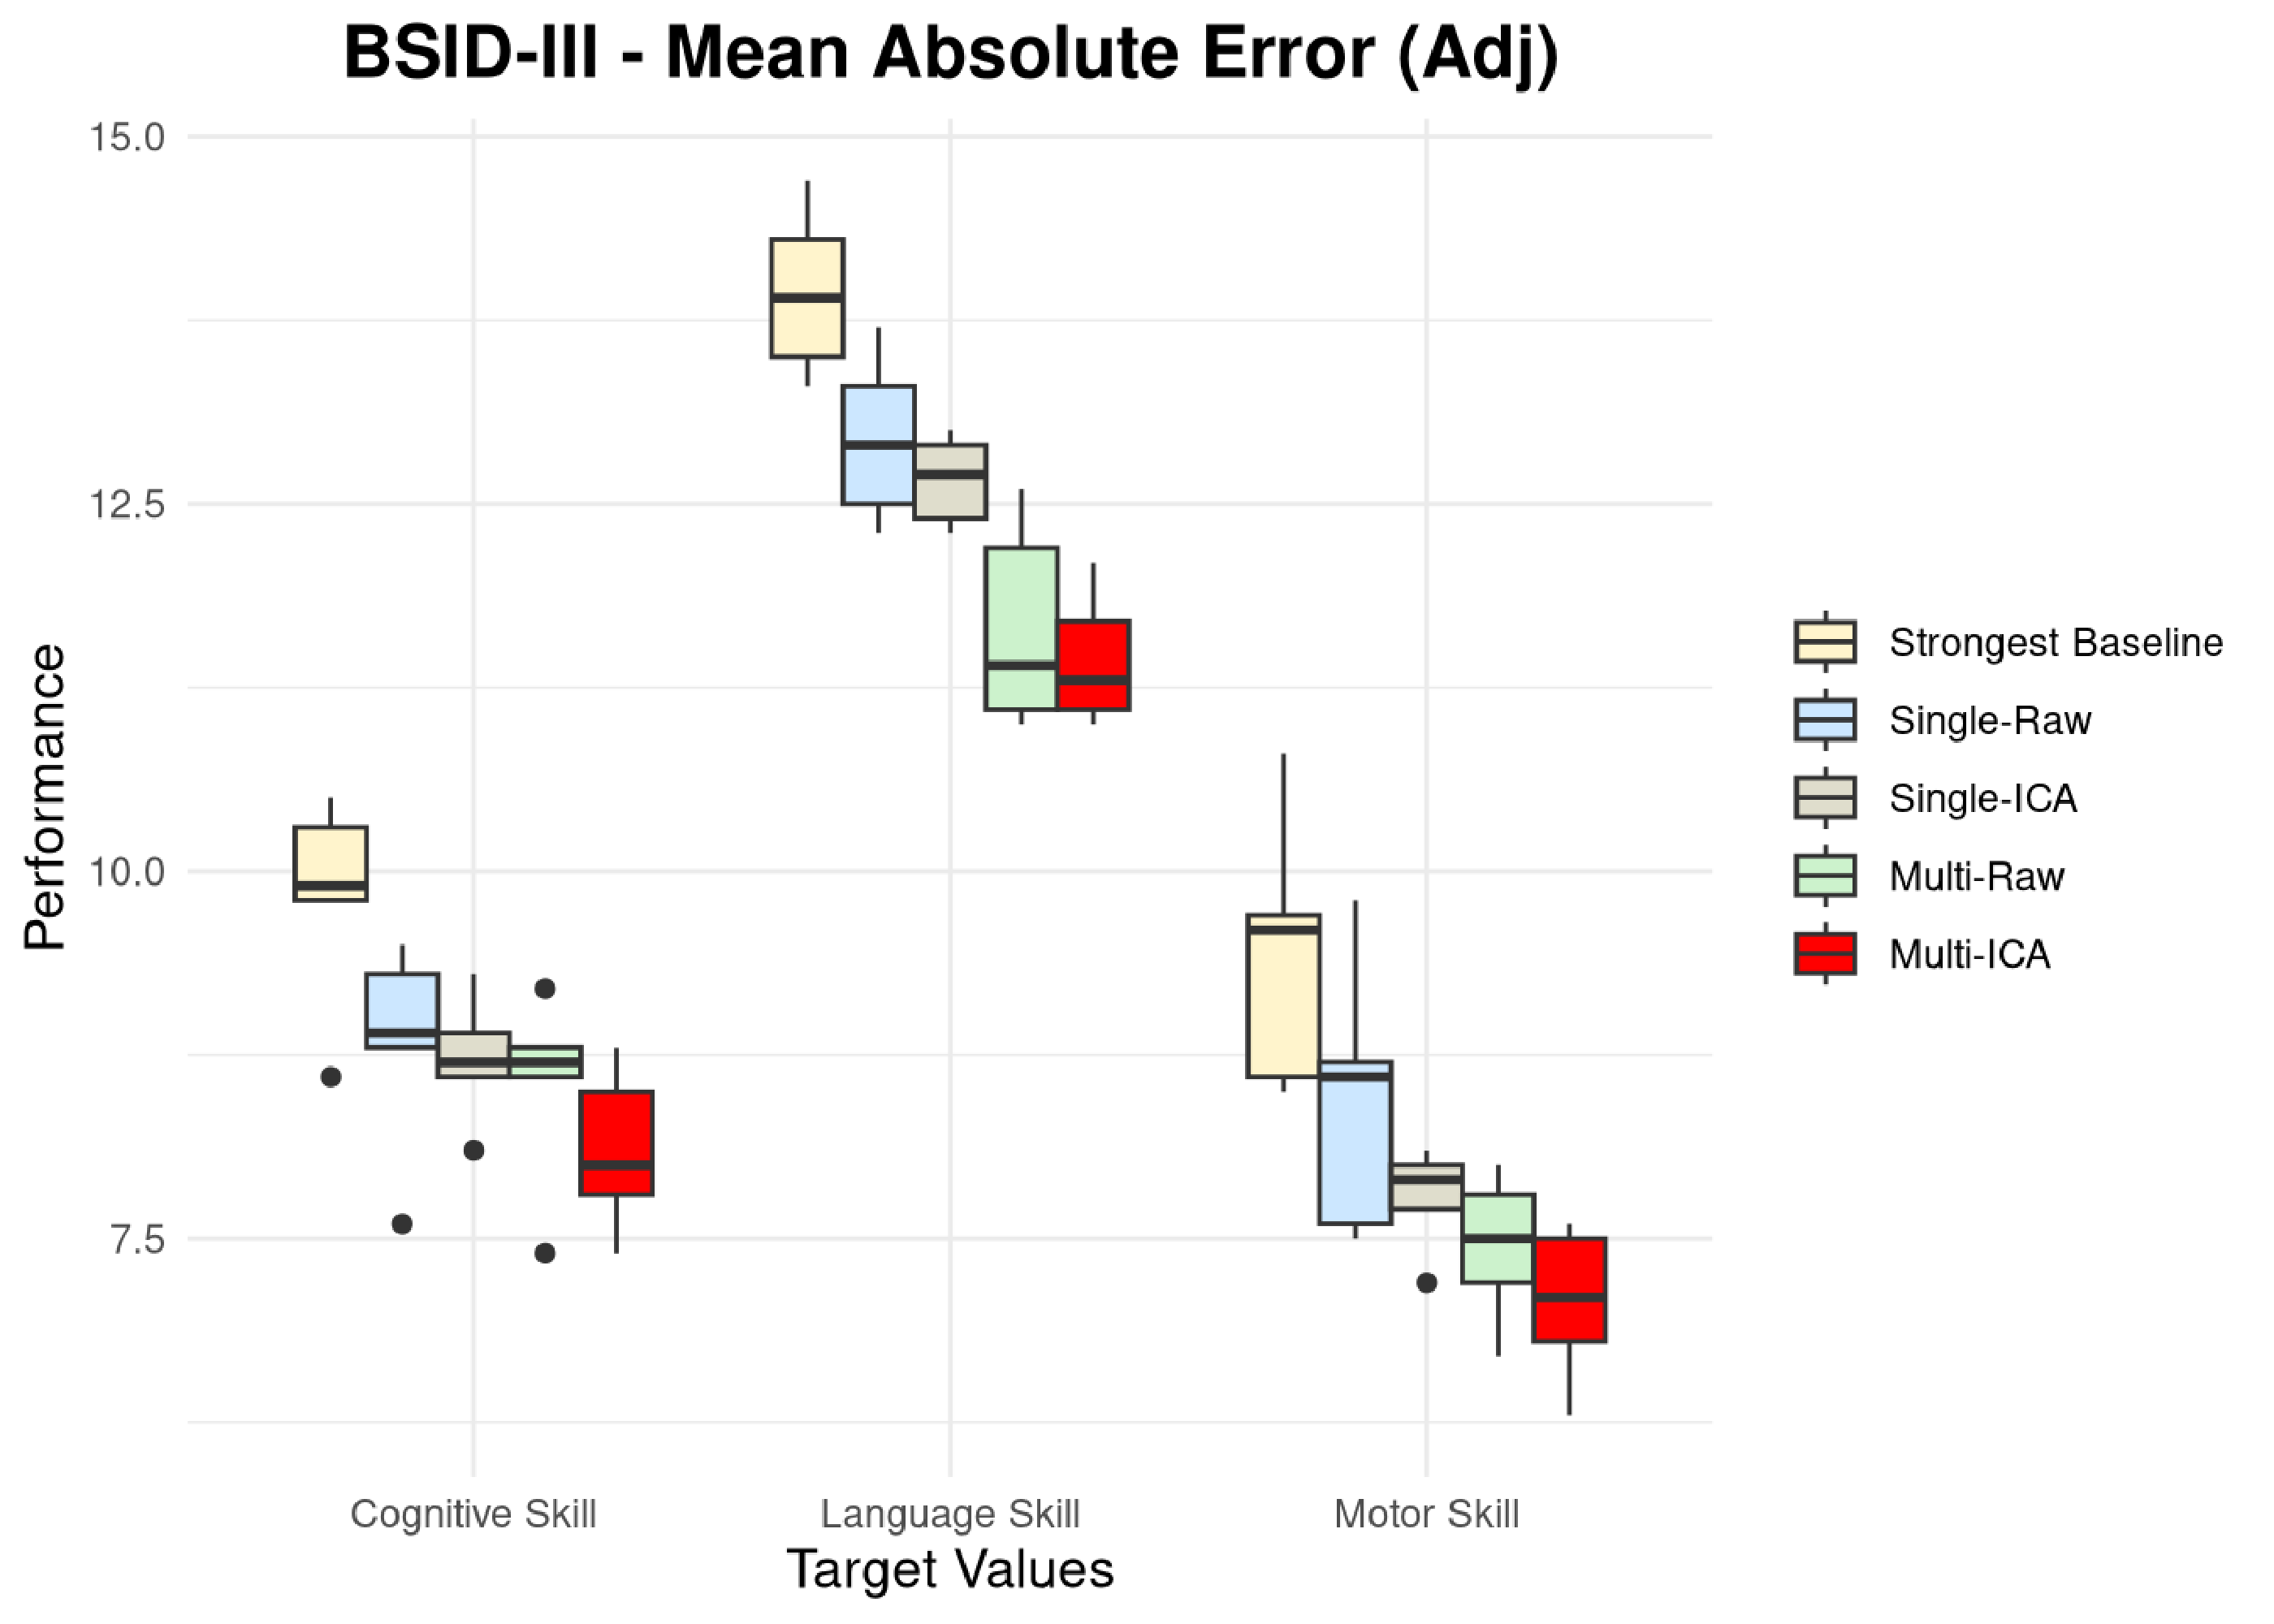
\includegraphics[width=\textwidth]{img/mae_overview.pdf}
    \end{minipage}
    \hfill
    \begin{minipage}{0.45\textwidth}
        \centering
        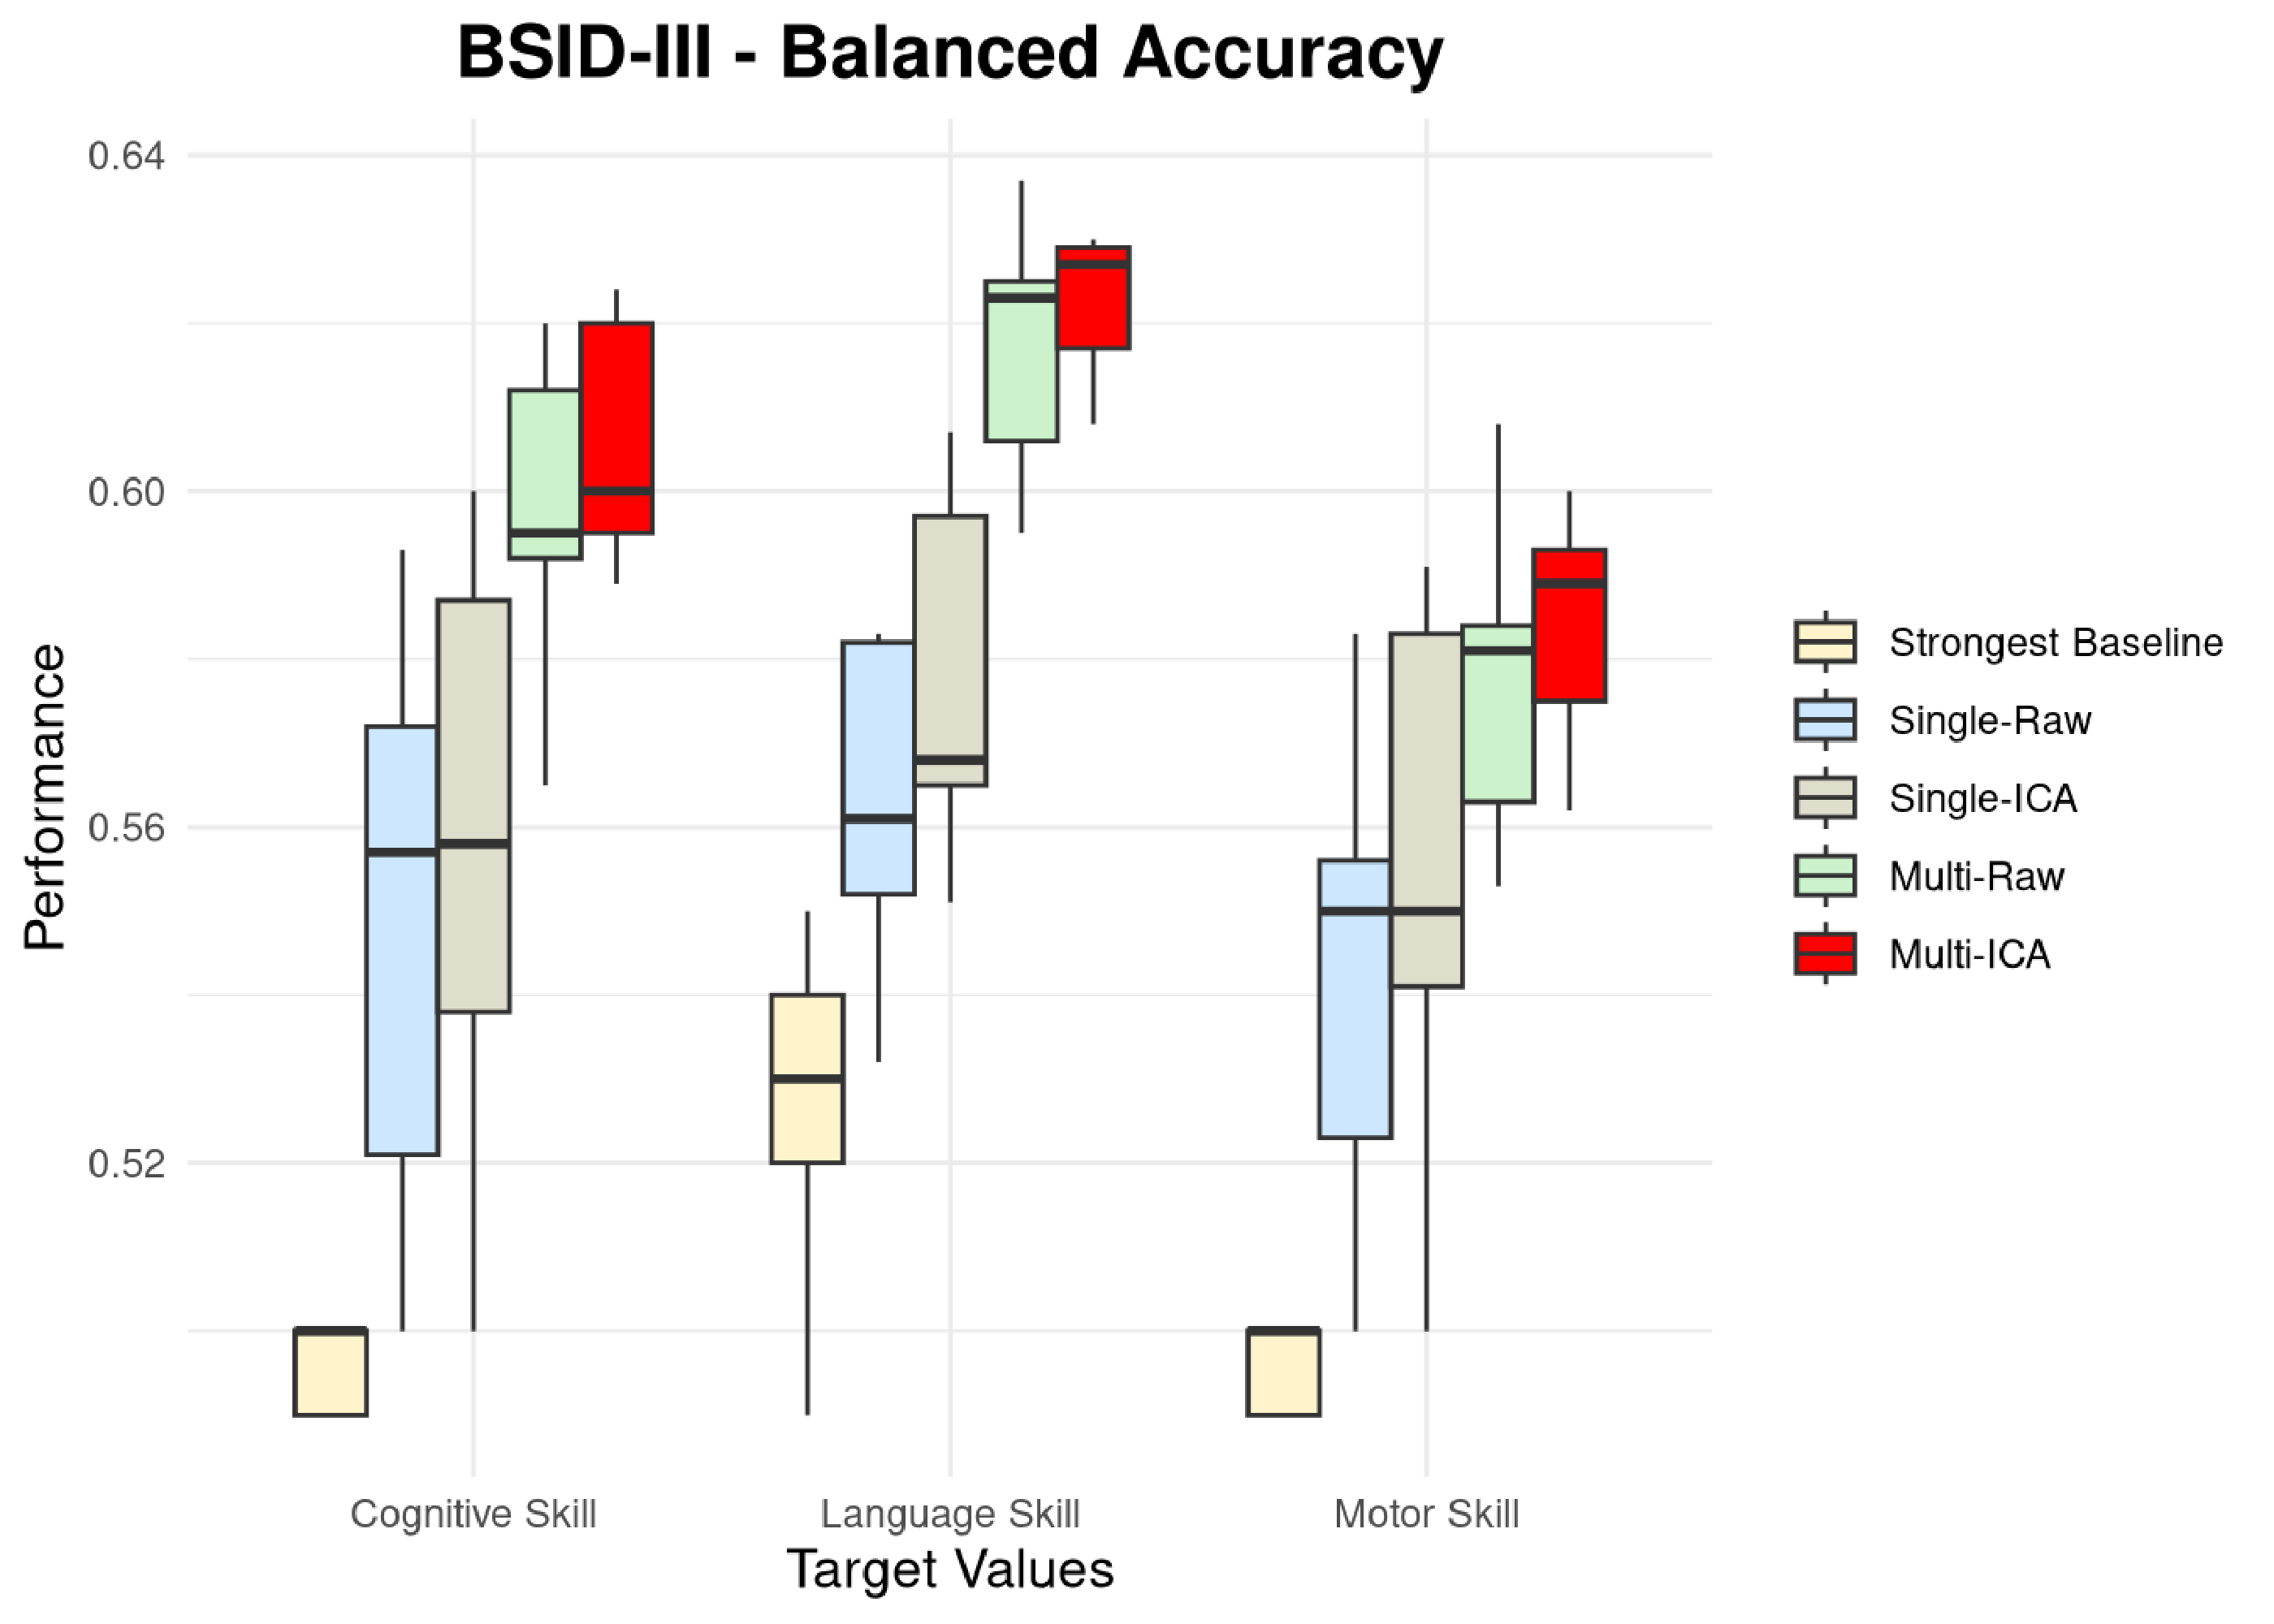
\includegraphics[width=\textwidth]{img/balacc_overview.pdf}
    \end{minipage}
    \caption{Overview of the models' predictive power via 5-fold cross-validation for BSID-III regression ($\text{MAE}_{adj}$) and classification ($\text{ACC}_{bal}$). The strongest baseline was taken to represent baseline performance. Performance by transfer-learning and 100 ICs was omitted due to no statistically significant performance changes.}
    \label{fig:overview}
\end{figure}

%\vspace{-1cm}

\subsection{Attribution Analysis}
\label{sec:interpretations}
%
The attribution analysis using IG-SQ revealed different brain regions whose spatiotemporal dynamics contribute to each developmental outcome (Figure~\ref{fig:interpretation}). For the risk of cognitive delay, activations were observed in the medial prefrontal cortex (coronal view), the thalamocortical circuit (sagittal and axial view) and the posterior parietal association cortex (sagittal view). These findings align with the neuroscience literature: identified brain regions are key to early sensory processing, attention, executive function, and spatial cognition, all foundational to normal cognitive development~\cite{mpfc}~\cite{thalamus}~\cite{ppc}. 
%
In Figure~\ref{fig:ica_int}, the network-level predictions are further explored. For example, IC5 closely resembles the Executive Control Network (ECN)\cite{Li2019}, a critical network for cognitive functions such as attention and decision-making. Its contribution to the general interpretation, as shown in Figure~\ref{fig:interpretation}, is evident through activations in the medial prefrontal cortex (mPFC), a hallmark region of the ECN.

\begin{figure}
    \centering
    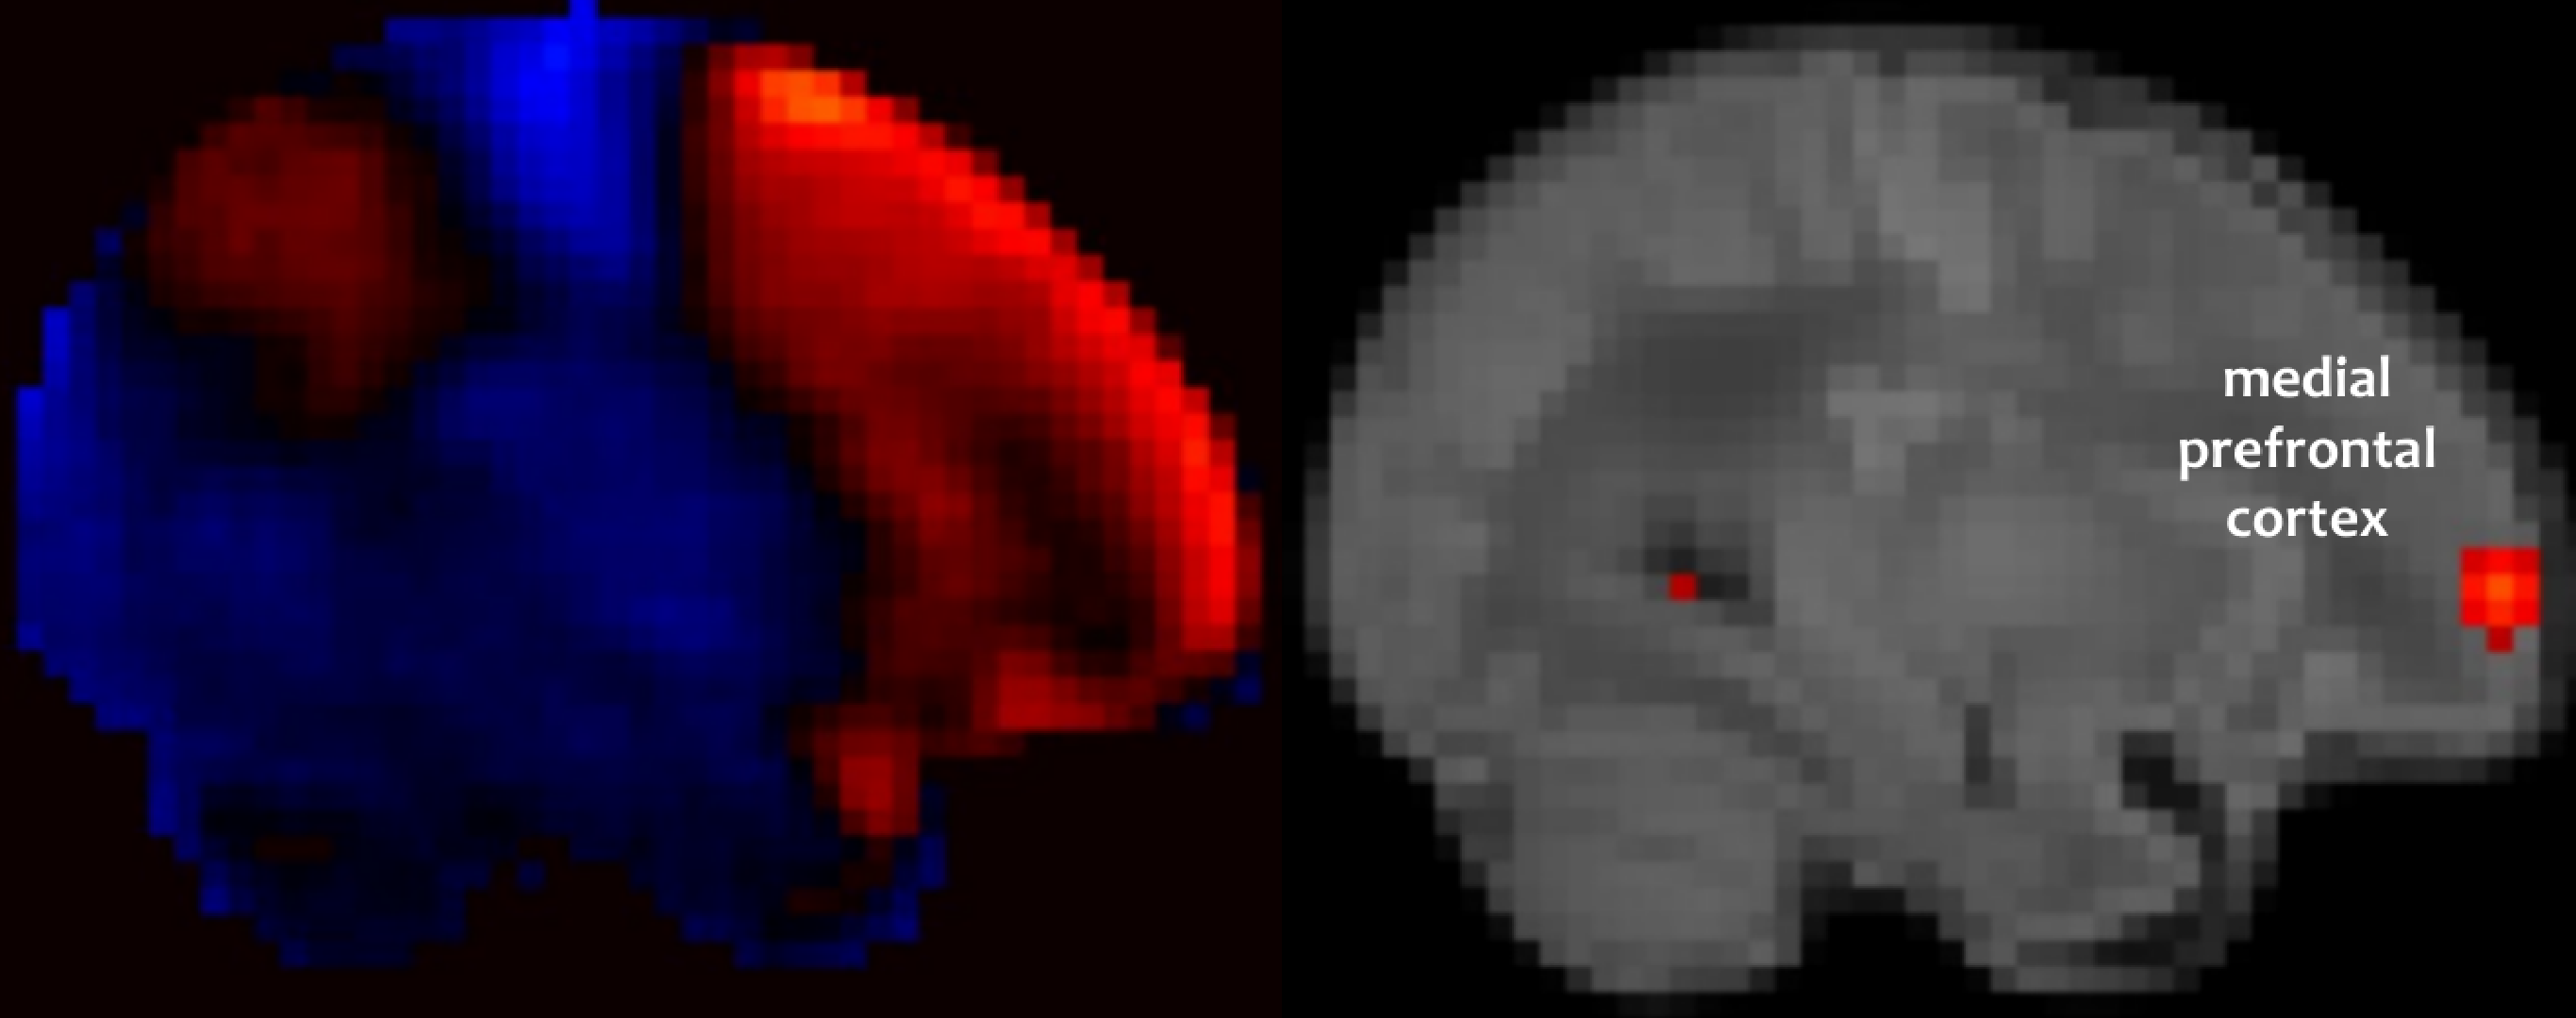
\includegraphics[width=0.6\linewidth]{img/ic_int.pdf}
    \caption{A glimpse into network-level interpretations, focusing on IC~5~(left) closely resembling the Executive Control Network~(ECN). We can see how this network adds to activation in the medial prefrontal cortex for prediction of cognitive delay (right).}
    \label{fig:ica_int}
\end{figure}

%
For the risk of linguistic delay (middle), activations in Wernicke's area align with its well-documented role in language comprehension and development~\cite{Binder2015}. Similarly, for motor skill delays (bottom), activations in the primary motor cortex and additional motor areas (SMAs) highlight their roles in gross and fine motor control and motor pattern learning, respectively~\cite{Graziano2006}~\cite{Tanji1994}. 

\begin{figure}[h]
    \centering
    \begin{minipage}{0.6\linewidth}
        \centering
        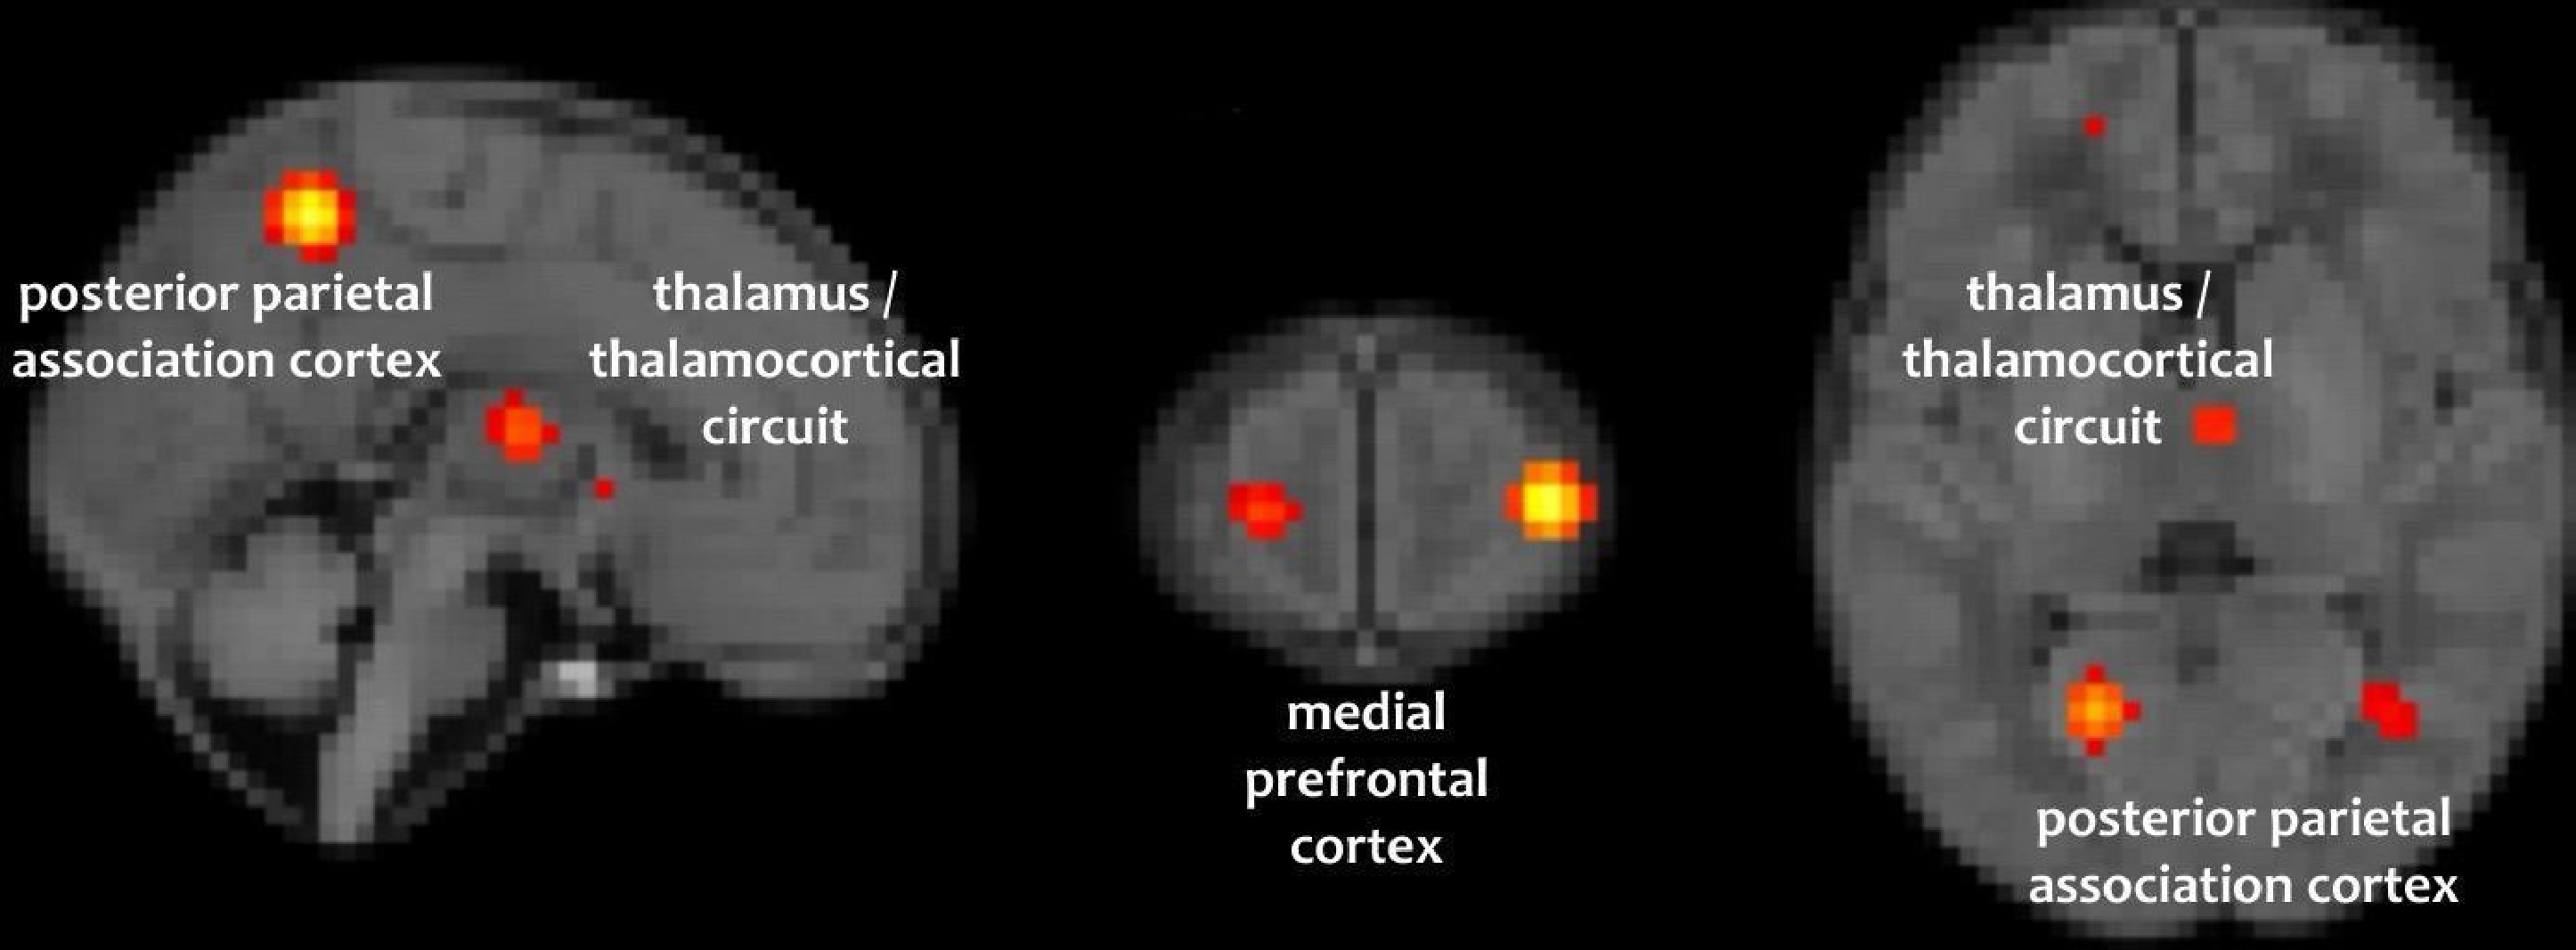
\includegraphics[width=\textwidth]{img/cog_int.pdf}
    \end{minipage}
    
    \vspace{0.2em}
    
    \begin{minipage}{0.6\linewidth}
        \centering
        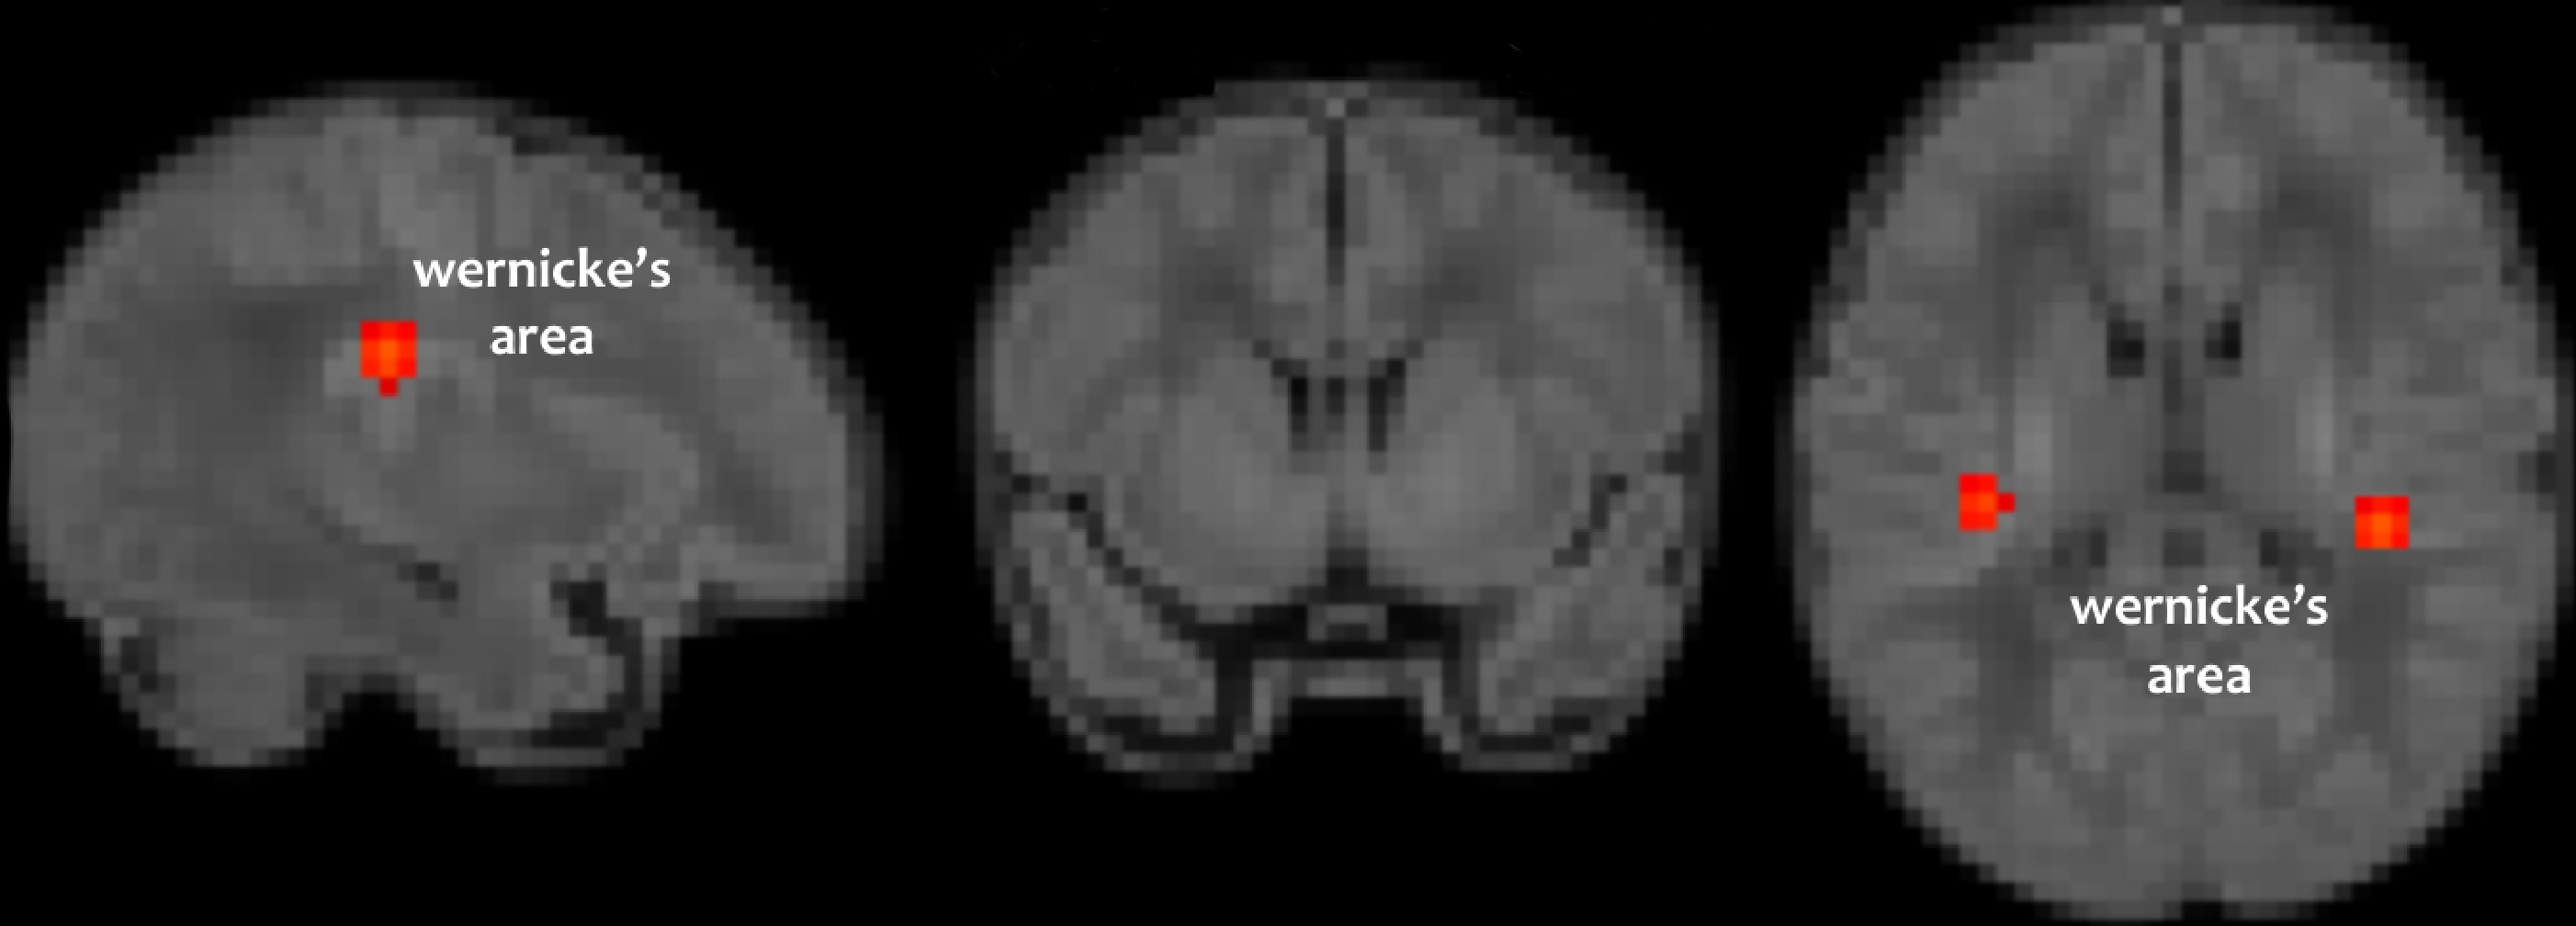
\includegraphics[width=\textwidth]{img/lang_int.pdf}
    \end{minipage}
    
    \vspace{0.2em}
    
    \begin{minipage}{0.6\linewidth}
        \centering
        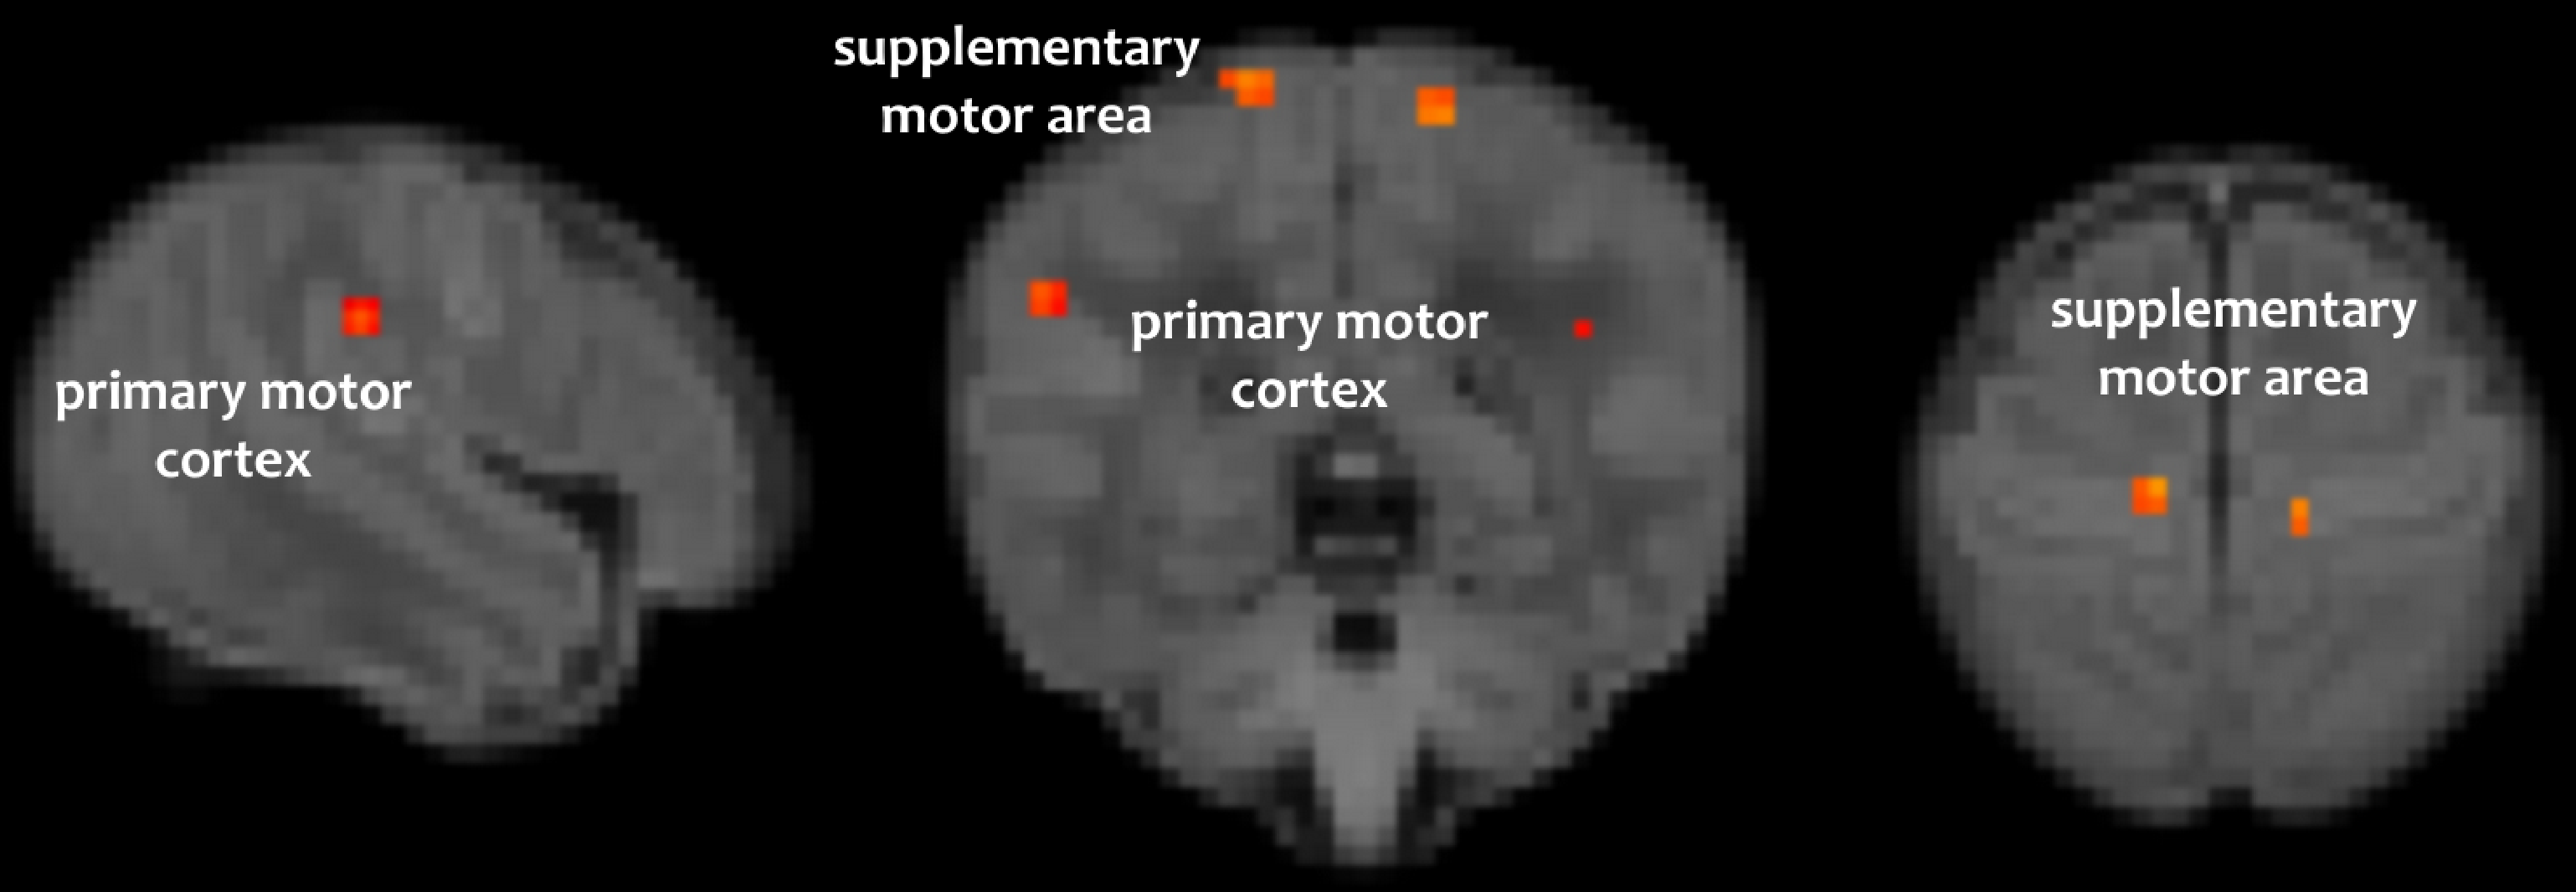
\includegraphics[width=\textwidth]{img/mot_int.pdf}
    \end{minipage}
    \caption{Interpretation maps with thresholded Integrated Gradients (IG) maps averaged across ICs for risk of cognitive (top), language (middle) and motor (bottom) delay.}
    \label{fig:interpretation}
\end{figure}

\section{Discussion}

\subsection{Interpretation of Model Findings}
This study demonstrates that integrating Group ICA-based dimensionality reduction with SwiFT significantly improves the predictions of neurodevelopmental outcomes from neonatal fMRI data. This is particularly relevant as our understanding of functional connectivity development in the prenatal and neonatal stages continues to expand \cite{Desrosiers2024Review}. By extracting biologically meaningful features via ICA and leveraging multi-label learning, the approach preserves critical neural information while reducing computational complexity. As seen in the comparative analysis, each form of SwiFT outperforms baselines by leveraging its attention-based architecture to effectively learn local and global spatiotemporal patterns in 4D fMRI data, underscoring the synergy between neuroscience-driven feature engineering and advanced machine learning \cite{TrendsCogSci2024Transformers,IEEETMI2024Swin}.
%

Results suggest that multi-label learning leads to improved performances compared to single-label learning in both fMRI volume-based models and IC-based models, and these improvements may stem from shared learning across developmental domains that allow models to capture complex and interrelated features of early brain development. Additionally, IC-based models outperformed fMRI volume-based models and highlighted the advantages of ICA in retaining biologically meaningful information while reducing noise. Naturally, the combination of ICA and multi-label learning further enhanced predictive power, and these findings reinforce the value of ICA as a preprocessing step, allowing the model to focus on key neural networks and achieve improved accuracy and efficiency. This targeted approach demonstrates the potential of integrating neuroscience-driven features with attention-based architectures for advancing neurodevelopmental research.
%

The attribution analysis using IG-SQ revealed distinct brain regions whose spatiotemporal dynamics contribute to each developmental outcome, and these findings reinforce the model's ability to capture neurobiologically meaningful spatiotemporal patterns. By integrating both spatial location and temporal dynamics of brain activity, the model effectively associates developmental delays with functional neural circuits. This alignment with established neuroscience underscores the robustness of our approach, demonstrating how machine learning can provide interpretable insights into the neural basis of developmental outcomes.

\subsection{Limitations and Future Directions}
%
Despite these accomplishments, limitations remain. The imbalanced nature of the data set poses a challenge and affects the reliability of the classification tasks. Although our approach partially mitigated this issue, future work should explore advanced strategies for handling data imbalances, such as oversampling or even synthetic data generation \cite{Zhang2024Preterm}. Additionally, further validation of ICA-extracted features as proxies for brain-network-level mechanisms is necessary to strengthen the biological interpretability of our findings, especially in the context of age-dependent functional development patterns \cite{Zhao2024AgeDependent}. In addition, expanding this framework to include datasets from other age groups, such as toddlers, children, and adults, could improve the generalizability of the model, especially when considering deviations from normative trajectories \cite{bioRxiv2024BrainAge}. Benchmarking against emerging foundation model challenges for brain MRI \cite{FOMO2025} and investigating the emergence of specialized circuits like social brain networks \cite{NatureHB2024Social} will provide further insights into the clinical utility of these models. Extending the multi-label learning paradigm to incorporate additional target variables, such as the Q-CHAT score for early autism screening, offers an exciting direction for future research and could be implemented into the current pipeline without major changes. Furthermore, adopting specialized architectures such as the ST-Transformer \cite{STTransformer2025} could better capture infant-specific anatomy. Finally, pretraining on adult data could provide a robust foundation for the model, but has shown no generalizability to neonates in our experiments. Since the use of small neonatal datasets increases the risk of overfitting, examining other pretraining paradigms than contrastive learning, such as Masked Image Modeling, may be beneficial \cite{MedImgAnal2024SSL,NatureComm2024Scaling}.

\section{Conclusion}
\label{sec:conclusion}
%
In this study, we demonstrate that SwiFT provides a significant improvement in evaluating neonatal fMRI data to predict early neurodevelopmental outcomes. By integrating multi-label learning and leveraging ICA-extracted features, we achieved enhanced predictive accuracy while improving model interpretability. These advances suggest that SwiFT has the potential to play a key role in the early detection of developmental delays, paving the way for personalized therapeutic interventions for at-risk newborns. The clinical relevance of such a model is strengthened by a study suggesting that therapeutic interventions to treat neurodevelopmental disorders may be more effective if done during the early stages of brain development~\cite{SVALINA2022}.
%

In conclusion, this work establishes a robust foundation for the advancement of predictive and interpretable models of neurodevelopment, aligning with the transformative impact of AI in pediatric neuroradiology \cite{RadiologyAI2024}. With continued refinement and access to diverse large-scale datasets, including high-risk extremely preterm populations \cite{Schmidbauer2024Outcome}, SwiFT holds significant potential for innovations in neuroscience and personalized medicine.

%\vspace{-.4cm}

\section*{Acknowledgements}
\label{sec:acknowledgements}
{%\small
This work was supported by the National Research Foundation of Korea(NRF) grant funded by the Korea government(MSIT) (No. 2021R1C1C1006503, RS-2023-00266787, RS-2023-00265406, RS-202400421268), by Creative-Pioneering Researchers Program through Seoul National University(No. 20020240057), by Semi-Supervised Learning Research Grant by SAMSUNG(No.A0426-20220118), by Identify the network of brain preparation steps for concentration Research Grant by LooxidLabs(No.33920230001), by Institute of Information \& communications Technology Planning \& Evaluation (IITP) grant funded by the Korea government(MSIT) [NO.RS-2021-II211343, Artificial Intelligence Graduate School Program (Seoul National University)] by the MSIT(Ministry of Science, ICT), Korea, under the Global Research Support Program in the Digital Field program(RS-2024-00421268) supervised by the IITP(Institute for Information \& Communications Technology Planning \& Evaluation), by the National Supercomputing Center with supercomputing resources including technical support(KSC-2023CRE-0568) and by the Ministry of Education of the Republic of Korea and the National Research Foundation of Korea (NRF - 2021S1A3A2A02090597), and by Artificial intelligence industrial convergence cluster development project funded by the Ministry of Science and ICT(MSIT, Korea) \& Gwangju Metropolitan City. This research used resources of: the Oak Ridge Leadership Computing Facility, a DOE Office of Science User Facility supported under Contract DE-AC05-00OR22725; the National Energy Research Scientific Computing Center, a DOE Office of Science User Facility using NERSC award NERSC DDR-ERCAP0030592 and DDR-GenAI, and ALCC-ERCAP0030659.
}

\begin{thebibliography}{4}

\bibitem{LI2024114168} Qiongling Li, Mingrui Xia, Debin Zeng, Yuehua Xu, Lianglong Sun, Xinyuan Liang, Zhilei Xu, Tengda Zhao, Xuhong Liao, Huishu Yuan, Ying Liu, Ran Huo, Shuyu Li, Yong He: Development of segregation and integration of functional connectomes during the first 1,000 days. Cell Reports 43, 114168 (2024)

%\bibitem{Xia2024} Xia, Y., Zhao, J., Xu, Y., Duan, D., Xia, M., Jeon, T., Ouyang, M., Chalak, L., Rollins, N., Huang, H., He, Y.: Development of sensorimotor-visual connectome gradient at birth predicts neurocognitive outcomes at 2 years of age. iScience 27, 108981 (2024)

%\bibitem{GONDOVA2023100170} Gondová, A., Neumane, S., Leprince, Y., Mangin, J.F., Arichi, T., Dubois, J: Predicting neurodevelopmental outcomes from neonatal cortical microstructure: A conceptual replication study. Neuroimage: Reports 3, 100170 (2023)

%\bibitem{Eyre2021} Eyre, M., Fitzgibbon, S. P., Ciarrusta, J., Cordero-Grande, L., Price, A. N., Poppe, T., Schuh, A., Hughes, E., O'Keeffe, C., Brandon, J., Cromb, D., Vecchiato, K., Andersson, J., Duff, E. P., Counsell, S. J., Smith, S. M., Rueckert, D., Hajnal, J. V., Arichi, T., O'Muircheartaigh, J., Batalle, D., Edwards, A. D.: The Developing Human Connectome Project: typical and disrupted perinatal functional connectivity. Brain 144, 2199--2213 (2021)

\bibitem{FITZGIBBON2020117303} Sean P. Fitzgibbon, Samuel J. Harrison, Mark Jenkinson, Luke Baxter, Emma C. Robinson, Matteo Bastiani, Jelena Bozek, Vyacheslav Karolis, Lucilio {Cordero Grande}, Anthony N. Price, Emer Hughes, Antonios Makropoulos, Jonathan Passerat-Palmbach, Andreas Schuh, Jianliang Gao, Seyedeh-Rezvan Farahibozorg, Jonathan O'Muircheartaigh, Judit Ciarrusta, Camilla O'Keeffe, Jakki Brandon, Tomoki Arichi, Daniel Rueckert, Joseph V. Hajnal, A. David Edwards, Stephen M. Smith, Eugene Duff, Jesper Andersson: The developing Human Connectome Project (dHCP) automated resting-state functional processing framework for newborn infants. NeuroImage 223, 117303 (2020)

\bibitem{Schuh2018} Schuh, Andreas, Makropoulos, Antonios, Robinson, Emma C., Cordero-Grande, Lucilio, Hughes, Emer, Hutter, Jana, Price, Anthony N, Murgasova, Maria, Teixeira, Rui Pedro A. G., Tusor, Nora, Steinweg, Johannes K., Victor, Suresh, Rutherford, Mary A., Hajnal, Joseph V., Edwards, A. David, Rueckert, Daniel: Unbiased construction of a temporally consistent morphological atlas of neonatal brain development. bioRxiv ,  (2018)

\bibitem{tustison_antsx_2021} Tustison, Nicholas J., Cook, Philip A., Holbrook, Andrew J., Johnson, Hans J., Muschelli, John, Devenyi, Gabriel A., Duda, Jeffrey T., Das, Sandhitsu R., Cullen, Nicholas C., Gillen, Daniel L., Yassa, Michael A., Stone, James R., Gee, James C., Avants, Brian B.: The {ANTsX} ecosystem for quantitative biological and medical imaging. Scientific Reports 11, 9068 (2021)

\bibitem{johnson2014using} Johnson, Samantha, Moore, Tamanna, Marlow, Neil: Using the Bayley-III to assess neurodevelopmental delay: which cut-off should be used?. Pediatric Research 75, 670--674 (2014)

\bibitem{KAWAHARA20171038} Jeremy Kawahara, Colin J. Brown, Steven P. Miller, Brian G. Booth, Vann Chau, Ruth E. Grunau, Jill G. Zwicker, Ghassan Hamarneh: BrainNetCNN: Convolutional neural networks for brain networks; towards predicting neurodevelopment. NeuroImage 146, 1038-1049 (2017)

\bibitem{he2020multi} He, Lili, Li, Hailong, Wang, Jinghua, Chen, Ming, Gozdas, Elveda, Dillman, Jonathan R, Parikh, Nehal A: A multi-task, multi-stage deep transfer learning model for early prediction of neurodevelopment in very preterm infants. Scientific Reports 10, 15072 (2020)

\bibitem{Miller2016} Miller, Karla L., Alfaro-Almagro, Fidel, Bangerter, Neal K., Thomas, David L., Yacoub, Essa, Xu, Junqian, Bartsch, Andreas J., Jbabdi, Saad, Sotiropoulos, Stamatios N., Andersson, Jesper L. R., Griffanti, Ludovica, Douaud, Gwena{\"e}lle, Okell, Thomas W., Weale, Peter, Dragonu, Iulius, Garratt, Steve, Hudson, Sarah, Collins, Rory, Jenkinson, Mark, Matthews, Paul M., Smith, Stephen M.: Multimodal Population Brain Imaging in the UK Biobank Prospective Epidemiological Study. Nature Neuroscience 19, 1523--1536 (2016)

\bibitem{ALFAROALMAGRO2018400} Fidel Alfaro-Almagro, Mark Jenkinson, Neal K. Bangerter, Jesper L.R. Andersson, Ludovica Griffanti, Gwenaëlle Douaud, Stamatios N. Sotiropoulos, Saad Jbabdi, Moises Hernandez-Fernandez, Emmanuel Vallee, Diego Vidaurre, Matthew Webster, Paul McCarthy, Christopher Rorden, Alessandro Daducci, Daniel C. Alexander, Hui Zhang, Iulius Dragonu, Paul M. Matthews, Karla L. Miller, Stephen M. Smith: Image processing and Quality Control for the first 10,000 brain imaging datasets from UK Biobank. NeuroImage 166, 400-424 (2018)

\bibitem{Hyvarinen1999} Hyvärinen, Aapo: Fast and Robust Fixed-Point Algorithms for Independent Component Analysis. IEEE Transactions on Neural Networks 10, 626--634 (1999)

\bibitem{Beckmann2004} Beckmann, Christian F., Smith, Stephen M.: Probabilistic Independent Component Analysis for Functional Magnetic Resonance Imaging. IEEE Transactions on Medical Imaging 23, 137--152 (2004)

\bibitem{Smith2014} Smith, Stephen M., Hyvärinen, Aapo, Varoquaux, Gaël, Miller, Karla L., Beckmann, Christian F.: Group-PCA for Very Large fMRI Datasets. NeuroImage 101, 738--749 (2014)

\bibitem{SMITH2013144} Stephen M. Smith, Christian F. Beckmann, Jesper Andersson, Edward J. Auerbach, Janine Bijsterbosch, Gwenaëlle Douaud, Eugene Duff, David A. Feinberg, Ludovica Griffanti, Michael P. Harms, Michael Kelly, Timothy Laumann, Karla L. Miller, Steen Moeller, Steve Petersen, Jonathan Power, Gholamreza Salimi-Khorshidi, Abraham Z. Snyder, An T. Vu, Mark W. Woolrich, Junqian Xu, Essa Yacoub, Kamil Uğurbil, David C. {Van Essen}, Matthew F. Glasser: Resting-state fMRI in the Human Connectome Project. NeuroImage 80, 144-168 (2013)

\bibitem{doi} Smith, S., Fox, P., Miller, K., Glahn, D., Fox, P., Mackay, C. , Filippini, N., Watkins, K., Toro, R., Laird, A., Beckmann, C.: Correspondence of the brain's functional architecture during activation and rest. Proceedings of the National Academy of Sciences 106, 13040-13045 (2009)

\bibitem{kim2023swiftswin4dfmri} Peter Yongho Kim, Junbeom Kwon, Sunghwan Joo, Sangyoon Bae, Donggyu Lee, Yoonho Jung, Shinjae Yoo, Jiook Cha, Taesup Moon: SwiFT: Swin 4D fMRI Transformer. arXiv preprint \url{https://arxiv.org/abs/2307.05916} (2023).

\bibitem{vanEssen2013HCP} Van Essen, David C, Smith, Stephen M, Barch, Deanna M, Behrens, Timothy EJ, Yacoub, Essa, Ugurbil, Kamil, Wu-Minn HCP Consortium: The Wu-Minn Human Connectome Project: an overview. Neuroimage 80, 62--79 (2013)

\bibitem{casey2018ABCD} Casey, Betty Jo, Cannonier, Tariq, Conley, May I, Cohen, Alexandra O, Barch, Deanna M, Heitzeg, Mary M, Soules, Mary E, Teslovich, Theresa, Dellarco, Danielle V, Garavan, Hugh, others: The adolescent brain cognitive development (ABCD) study: imaging acquisition across 21 sites. Developmental Cognitive Neuroscience 32, 43--54 (2018)

\bibitem{miller2016UKBiobank} Miller, Karla L, Alfaro-Almagro, Fidel, Bangerter, Neal K, Thomas, David L, Yacoub, Essa, Xu, Junqian, Bartsch, Andreas J, Jbabdi, Saad, Sotiropoulos, Stamatios N, Andersson, Jesper LR, others: Multimodal population brain imaging in the UK Biobank prospective epidemiological study. Nature Neuroscience 19, 1523--1536 (2016)

\bibitem{alfaro2018UKBiobank} Alfaro-Almagro, Fidel, Jenkinson, Mark, Bangerter, Neal K, Andersson, Jesper LR, Griffanti, Ludovica, Douaud, Gwena{\"e}lle, Sotiropoulos, Stamatios N, Jbabdi, Saad, Hernandez-Fernandez, Moises, Vallee, Emmanuel, others: Image processing and quality control for the first 10,000 brain imaging datasets from UK Biobank. Neuroimage 166, 400--424 (2018)

\bibitem{dave2022TCLR} Dave, Ishan, Gupta, Rohit, Rizve, Mamshad Nayeem, Shah, Mubarak: TCLR: Temporal contrastive learning for video representation. Computer Vision and Image Understanding 219, 103406 (2022)

\bibitem{GAL2022118920} Shachar Gal, Niv Tik, Michal Bernstein-Eliav, Ido Tavor: Predicting individual traits from unperformed tasks. NeuroImage 249, 118920 (2022)

\bibitem{lin2018focallossdenseobject} Tsung-Yi Lin, Priya Goyal, Ross Girshick, Kaiming He, Piotr Dollár: Focal Loss for Dense Object Detection. arXiv preprint \url{https://arxiv.org/abs/1708.02002} (2018).

\bibitem{He2020} He, L., Li, H., Wang, J., Chen, M., Gozdas, E., Dillman, J., Parikh, N.: A multi-task, multi-stage deep transfer learning model for early prediction of neurodevelopment in very preterm infants. Scientific Reports 10, 15072 (2020)

\bibitem{captum1} Rahman, Md Monirul, Mahmood, Usama, Lewis, Nate, Gazula, Hima, Fedorov, Andrei, Fu, Zhifei, Calhoun, Vince D., Plis, Sergey M.: Interpreting models interpreting brain dynamics. Scientific Reports 12, 12023 (2022)

\bibitem{mpfc} Mair, R.  Francoeur, M.  Krell, E.  Gibson, B.: Where Actions Meet Outcomes: Medial Prefrontal Cortex, Central Thalamus, and the Basal Ganglia. Frontiers in Behavioral Neuroscience. 16, 1662--5153 (2022)

\bibitem{thalamus} Benarroch, Eduardo E., Benarroch, Eduardo E.: 477Thalamus and Thalamocortical Interactions. In: Neuroscience for Clinicians: Basic Processes, Circuits, Disease Mechanisms, and Therapeutic Implications, pp. . Oxford University Press (2021)

\bibitem{ppc} Shomstein, S.: Cognitive functions of the posterior parietal cortex: top-down and bottom-up attentional control. Frontiers in Integrative Neuroscience. 6, 1662--5145 (2012)

\bibitem{Li2019} Li, Chunlei, Deng, Yanjun, He, Yunhan, Zhai, Haichao, Jia, Fucai: The development of brain functional connectivity networks revealed by resting-state functional magnetic resonance imaging. Neural Regeneration Research 14, 1419--1429 (2019)

\bibitem{Binder2015} Binder, Jeffrey R.: The Wernicke area: Modern evidence and reinterpretation. Neurology 85, 15-21 (2015)

\bibitem{Graziano2006} Graziano, Michael S. A.: The organization of behavioral repertoire in motor cortex. Annual Review of Neuroscience 29, 105-134 (2006)

\bibitem{Tanji1994} Tanji, Jun, Shima, Keisetsu: Role of supplementary motor area cells in planning and executing sequential movements. Brain Research 619, 260-263 (1994)

\bibitem{KAN2022} Kan, X., Dai, W., Cui, H., Zhang, Z., Guo, Y., Yang, C.: Brain Network Transformer, In: Advances in Neural Information Processing Systems 35, pp. 25586--25599. Curran Associates, Inc. (2022)

\bibitem{CHEN2016} Chen, Tianqi, Guestrin, Carlos: XGBoost: A Scalable Tree Boosting System. In: Proceedings of the 22nd ACM SIGKDD International Conference on Knowledge Discovery and Data Mining, pp. 785–794. Association for Computing Machinery (2016)

\bibitem{BECKMANN2009S148} Beckmann, C., Mackay, C., Filippini, N., Smith, S.: Group comparison of resting-state FMRI data using multi-subject ICA and dual regression. NeuroImage 47, S148 (2009)

\bibitem{SVALINA2022} Matthew N. Svalina, Christian A. Cea-Del Rio, J. Keenan Kushner, Abigail Levy, Serapio M. Baca, E. Mae Guthman, Maya Opendak, Regina M. Sullivan, Diego Restrepo, Molly M. Huntsman: Basolateral Amygdala Hyperexcitability Is Associated with Precocious Developmental Emergence of Fear-Learning in Fragile X Syndrome. Journal of Neuroscience, 42(38): 7294-7308 (2022). \url{https://doi.org/10.1523/JNEUROSCI.1776-21.2022}.

\bibitem{Sun2024NatureBME} Sun, L., et al.: A foundation model for enhancing magnetic resonance images and downstream segmentation, registration and diagnostic tasks. Nature Biomedical Engineering (2024)

\bibitem{Rahman2024BrainLM} Rahman, M. M., et al.: BrainLM: A Foundation Model for fMRI Data Analysis. ICLR/arXiv (2024)

\bibitem{Zhang2024Connectome} Zhang, H., et al.: A Foundation Model for Brain Connectomes. arXiv (2024)

\bibitem{Smith2024SharedBlueprint} Smith, S. M., et al.: Shared blueprint in brain development across different functional areas. PNAS (2024)

\bibitem{Zhao2024AgeDependent} Zhao, T., et al.: Age-dependent functional development pattern in neonatal brain: An fMRI-based brain entropy study. NeuroImage (2024)

\bibitem{Desrosiers2024Review} Desrosiers, M., et al.: Functional connectivity development in the prenatal and neonatal stages measured by fMRI: A systematic review. Neuroscience \& Biobehavioral Reviews (2024)

\bibitem{bioRxiv2024BrainAge} bioRxiv: Brain age prediction and deviations from normative trajectories in the neonatal connectome. bioRxiv (2024)

\bibitem{Schmidbauer2024Outcome} Schmidbauer, M., et al.: Quantitative MRI for Neurodevelopmental Outcome Prediction in Neonates Born Extremely Premature. Clinical Neuroradiology (2024)

\bibitem{Zhang2024Preterm} Zhang, Y., et al.: Predicting neurodevelopmental outcomes in extremely preterm neonates using synthetic MRI. Frontiers in Neuroscience (2024)

\bibitem{NatureMedicine2024Foundation} Nature Medicine: Foundation models for medical imaging. Nature Medicine (2024)

\bibitem{SLIMBrain2024} SLIM-Brain: Sample-efficient, Low-memory fMRI Foundation Model for Human Brain. arXiv (2024)

\bibitem{LancetDigitalHealth2024} Lancet Digital Health: Potential and pitfalls of foundation models in medical imaging. Lancet Digital Health (2024)

\bibitem{FOMO2025} FOMO Challenge: Foundation Model Challenge for Brain MRI. MICCAI (2025)

\bibitem{STTransformer2025} ST-Transformer: Spatio-Temporal Transformer for Neonatal MRI. ICLR (2025)

\bibitem{NatureComm2024Scaling} Nature Communications: Self-supervised learning for large-scale brain imaging. Nature Communications (2024)

\bibitem{MedImgAnal2024SSL} Medical Image Analysis: Contrastive learning and reconstruction-based pretraining for fMRI. Medical Image Analysis (2024)

\bibitem{NatureHB2024Social} Nature Human Behaviour: Emergence of social brain networks in early infancy. Nature Human Behaviour (2024)

\bibitem{IEEETMI2024Swin} IEEE TMI: 4D-Swin: Hierarchical Vision Transformer for 4D Medical Image Segmentation. IEEE TMI (2024)

\bibitem{RadiologyAI2024} Radiology: AI: Transformative impact of AI in pediatric neuroradiology. Radiology: AI (2024)

\bibitem{TrendsCogSci2024Transformers} Trends in Cognitive Sciences: From local circuits to global models: Transformers in neuroscience. Trends in Cognitive Sciences (2024)

\end{thebibliography}
\end{document}
